\documentclass[12pt,letterpaper]{article}
\usepackage[utf8]{inputenc}
\usepackage[T1]{fontenc}
\usepackage[spanish]{babel}
\usepackage{lmodern, microtype}
\usepackage{amsmath, amssymb, amsthm}
\usepackage{chngcntr, listings}
\usepackage{graphicx, tikz, float, xcolor}
\usepackage{booktabs, array, colortbl, enumitem}
\usepackage{geometry, fancyhdr, titlesec, tocloft}
\usepackage[normalem]{ulem}
\usepackage{caption}
\usepackage[hidelinks]{hyperref}

\geometry{margin=2.5cm, top=2.5cm, bottom=2.5cm}

\newcommand{\asig}{\leftarrow}
\definecolor{navyblue}{RGB}{20, 50, 100}
\definecolor{headbg}  {RGB}{228, 236, 250}

\titleformat{\section}
  {\large\bfseries\color{navyblue}}
  {\thesection.}{0.5em}{}
  [\vspace{2pt}\textcolor{navyblue}{\titlerule[0.7pt]}]
\titlespacing*{\section}{0pt}{22pt}{10pt}

\titleformat{\subsection}
  {\normalsize\bfseries\color{navyblue!85!black}}
  {\thesubsection}{0.5em}{}
\titlespacing*{\subsection}{0pt}{14pt}{5pt}

\titleformat{\subsubsection}
  {\normalsize\bfseries}
  {\thesubsubsection}{0.5em}{}
\titlespacing*{\subsubsection}{0pt}{12pt}{4pt}

\titleformat{\paragraph}[runin]
  {\normalsize\bfseries\itshape}{}{0pt}{}[\enspace]
\titlespacing*{\paragraph}{0pt}{8pt}{4pt}

\pagestyle{fancy}
\fancyhf{}
\fancyhead[L]{%
  \small\textit{\textcolor{navyblue}{Análisis de Cardiotocografía Fetal mediante Clustering}}}
\fancyhead[R]{\small\textcolor{navyblue}{\thepage}}
\renewcommand{\headrulewidth}{0.5pt}
\makeatletter
\renewcommand{\headrule}{%
  \vbox to 0pt{%
    \hbox to\headwidth{\color{navyblue}\leaders\hrule height\headrulewidth\hfill}%
    \vss}}
\makeatother

\renewcommand{\cftsecfont}{\bfseries\color{navyblue}}
\renewcommand{\cftsecpagefont}{\bfseries\color{navyblue}}
\setlength{\cftbeforesecskip}{5pt}
\setlength{\cftbeforesubsecskip}{1pt}

\renewcommand{\arraystretch}{1.30}
\setlength{\tabcolsep}{6pt}
\captionsetup{font=small, labelfont={bf,color=navyblue}, skip=5pt}

\begin{document}
\begin{titlepage}
  \thispagestyle{empty}
  %--------------- COMANDO LINEA----------------->
  \newcommand{\linea}{\rule{\linewidth}{0.5mm}}                 
  \center
  %<<<<<<<<<<<<<<<<<<<<<<<<<<<<<<<<<<<<<<<<<<<

  %Add logos
  
\includegraphics[width=0.24\textwidth]{~/unam_logo.png} \hspace{1.5cm}
  
\includegraphics[width=0.25\textwidth]{~/fc_logo.png} \\[1cm]
  \textbf{\Large UNIVERSIDAD NACIONAL AUTÓNOMA}\\[3mm]
  \textbf{\Large DE MÉXICO} \\[6mm]
  \textit{\Large Facultad de Ciencias}

  \vfill

  %---------------TÍTULO----------------->
  \linea
  \vfill \vspace{1cm}
  \textbf{\Large Reconocimiento de Patrones y Aprendizaje Automatizado}\\[1.1cm]
  \textbf{\Large Proyecto Final}\\[0.5cm]
  \linea \\
  \vfill
  \vspace{0.7cm}
  %Title of the Research
  \textbf{\Large  Presentación}\\[6mm]
  %<<<<<<<<<<<<<<<<<<<<<<<<<<<<<<<<<<<<<<<<<<<

  %Team
  \vfill
  \textit{\small Presenta:}\\
  \textbf{\large \textbf{Hernández Zavala Ana Sofía}}\\[3mm]
  \textbf{\large \textbf{Ramírez Juárez María Fernanda}}\\[3mm]
  \textbf{\large \textbf{Rojo Peña Manuel Ianluck}}\\[3mm]

  %Profesor y Grupo
  \textit{\small Profesor:}\\
  \textbf{Sergio Rodolfo Cruz Gómez}\\[2mm]
  \textit{\small Ayudantes:}\\
  \textbf{Gustavo Adolfo Garduño Martínez}\\[1mm]
  \textbf{Julio César Misael Monroy Gónzalez}\\[1mm]
  \small Grupo: 7142, 2026-2\\[3mm]
  \vfill

  %Fecha or Date
  \textit{\small Fecha de entrega:}\\
         {\large 8 de abril, 2026}
         
\end{titlepage}


\newpage
\tableofcontents
\newpage

%%%%%%%%%%%%%%%%%%%%%%%%%%%%%%%%%%
\section{Introducción}
%%%%%%%%%%%%%%%%%%%%%%%%%%%%%%%%%%

La mortalidad infantil y materna representa uno de los indicadores más sensibles del nivel de
desarrollo humano. Los Objetivos de Desarrollo Sostenible de las Naciones Unidas establecen
como meta para 2030 la eliminación de las muertes prevenibles de recién nacidos, mientras que
en 2017 aproximadamente 295{,}000 mujeres fallecieron durante o tras el embarazo,
concentrándose el 94\,\% de esos casos en entornos de bajos recursos.

En este contexto, la Cardiotocografía (CTG) emerge como herramienta diagnóstica accesible,
no invasiva y de bajo costo que permite monitorear el estado de salud fetal durante la gestación.
Mediante el análisis de pulsos de ultrasonido, un equipo CTG registra la frecuencia cardíaca
fetal (FCF), los movimientos del feto y las contracciones uterinas.

El presente proyecto aplica técnicas de \textbf{clustering no supervisado} sobre un conjunto de
registros CTG para identificar agrupaciones naturales en el comportamiento fisiológico fetal,
y complementa el análisis con \textbf{modelos de clasificación supervisada} para predecir el
estado de salud fetal a partir de las mismas variables. A lo largo de las secciones exploramos
el preprocesamiento, la implementación de tres algoritmos de agrupamiento (K-Means++,
DBSCAN y GMM), tres clasificadores (KNN, Árbol de Decisión y MLP) y la comparación de
resultados con métricas internas, externas y de clasificación.

%%%%%%%%%%%%%%%%%%%%%%%%%%%%%%%%%%
\section{Participantes}
%%%%%%%%%%%%%%%%%%%%%%%%%%%%%%%%%%

El equipo está integrado por tres estudiantes de la Facultad de Ciencias de la UNAM
(Grupo 7142, semestre 2026-2), cada uno con un rol claramente delimitado:

\begin{itemize}[leftmargin=1.8cm]
  \item \textbf{Hernández Zavala Ana Sofía} (Lic. Matemáticas Aplicadas). Especialista en preprocesamiento de datos. Responsable de la auditoría, limpieza, normalización y transformación del dataset para dejarlo listo para los modelos.
  \item \textbf{Ramírez Juárez María Fernanda} (Lic. Ciencia de Datos). Analista de modelos. Encargada de implementar y evaluar los modelos de clustering e implementar las métricas de evaluación internas y externas.
  \item \textbf{Rojo Peña Manuel Ianluck} (Ing. Sistemas Computacionales). Líder de equipo. Coordinador del proyecto y responsable de los modelos de clasificación supervisada.
\end{itemize}

%%%%%%%%%%%%%%%%%%%%%%%%%%%%%%%%%%
\section{Descripción del Problema}
%%%%%%%%%%%%%%%%%%%%%%%%%%%%%%%%%%

\subsection{Contexto y motivación}

Abordar el análisis de registros de cardiotocografía desde una perspectiva de aprendizaje
no supervisado resulta especialmente interesante porque, a diferencia de la clasificación
supervisada, el clustering explora la estructura \textit{natural} de los datos sin imponer
categorías a priori. Esto permite descubrir agrupaciones que no necesariamente coincidan
con las clasificaciones diagnósticas convencionales.

\subsection{Descripción del problema}

El dataset contiene 2{,}126 registros de exámenes CTG, cada uno descrito por 21 variables
numéricas relacionadas con la dinámica cardíaca fetal y propiedades estadísticas del
histograma de frecuencia. Cada registro cuenta además con una etiqueta de clase asignada
por tres obstetras expertos que categoriza el estado fetal como \textbf{Normal},
\textbf{Sospechoso} o \textbf{Patológico}. Esta etiqueta no participa en el entrenamiento
de los modelos de clustering, aunque sí sirve como referencia externa para evaluar la
coherencia clínica de los grupos descubiertos.

\subsection{Justificación del dataset}

Seleccionamos el dataset \textit{Fetal Health Classification} (Kaggle, basado en Ayres de
Campos et al., 2000) por tres razones complementarias. Primero, el impacto social de
aplicar ciencias de la computación a la salud perinatal. Segundo, la naturaleza técnicamente
limpia pero desafiante del conjunto: variables puramente numéricas sin valores faltantes
permiten centrar los esfuerzos en la experimentación algorítmica. Tercero, la coexistencia
de variables con magnitudes radicalmente distintas (frecuencia cardíaca basal entre 106 y
159\,lpm frente a tasas de aceleración en milésimas de segundo) ofrece un entorno real
para evaluar técnicas de estandarización y reducción de dimensionalidad.

\subsection{Objetivo general}

Aplicar y comparar tres métodos de clustering sobre el dataset CTG para identificar
agrupaciones naturales, evaluar su coherencia interna mediante métricas especializadas,
contrastar los resultados con las categorías diagnósticas de referencia, y complementar
con clasificadores supervisados para determinar en qué medida el aprendizaje automático
es capaz de recuperar la estructura clínica subyacente.

%%%%%%%%%%%%%%%%%%%%%%%%%%%%%%%%%%
\section{Descripción del Dataset}
%%%%%%%%%%%%%%%%%%%%%%%%%%%%%%%%%%

\subsection{Fuente y dimensiones}

El dataset proviene de Kaggle bajo el título \textit{Fetal Health Classification}. Su origen
científico es el estudio de Ayres de Campos et al.\ (2000), publicado en el
\textit{Journal of Maternal-Fetal Medicine}. Está compuesto por \textbf{2{,}126 observaciones}
y \textbf{22 columnas}: 21 variables de entrada derivadas del análisis CTG y una columna
\texttt{fetal\_health} con la etiqueta clínica. No existen valores faltantes.

\subsection{Variables de entrada}

Todas las variables son numéricas. Dentro del conjunto conviven variables continuas
(aceleraciones, movimientos, contracciones, desaceleraciones) y variables discretas
(estadísticos del histograma de FCF: ancho, mínimo, máximo, picos, ceros, moda, media,
mediana, varianza). La Tabla~\ref{tab:variables} resume las más relevantes.

\begin{table}[H]
\centering
\caption{Selección de variables del dataset CTG con rango aproximado.}
\label{tab:variables}
\footnotesize
\begin{tabular}{lllp{5.8cm}}
\toprule
\rowcolor{headbg}
\textbf{Variable} & \textbf{Tipo} & \textbf{Rango aprox.} & \textbf{Observaciones clave} \\
\midrule
\texttt{baseline\_value}       & Discreta  & 106--159 bpm   & FCF basal; mayor magnitud absoluta del dataset \\
\texttt{accelerations}         & Continua  & 0.000--0.018   & Alta presencia de ceros; rango reducido \\
\texttt{fetal\_movement}       & Continua  & 0.000--0.481   & Distribución fuertemente asimétrica \\
\texttt{severe\_decelerations} & Continua  & 0.000--0.001   & Casi constante en 0.0 (solo 5 valores distintos) \\
\texttt{abnormal\_short\_term\_variability} & Discreta & 16--87\,\% & Buen rango de variación \\
\texttt{histogram\_mode / mean / median} & Discreta & 71--167 & Multicolinealidad elevada entre los tres \\
\texttt{histogram\_variance}   & Discreta  & 0--215         & Alta dispersión; outliers extremos \\
\texttt{histogram\_tendency}   & Discreta  & $-1,\,0,\,1$   & Variable ordinal categórica codificada \\
\bottomrule
\end{tabular}
\end{table}

\subsection{Variable objetivo y distribución de clases}

La columna \texttt{fetal\_health} toma tres valores: $1=\text{Normal}$, $2=\text{Sospechoso}$,
$3=\text{Patológico}$. Su distribución está marcadamente desbalanceada: la clase Normal
concentra aproximadamente el 78\,\% de los registros, mientras que Sospechoso y Patológico
representan el 14\,\% y el 8\,\% restantes (Figura~\ref{fig:distribucion_clases}).

\begin{figure}[H]
  \centering
  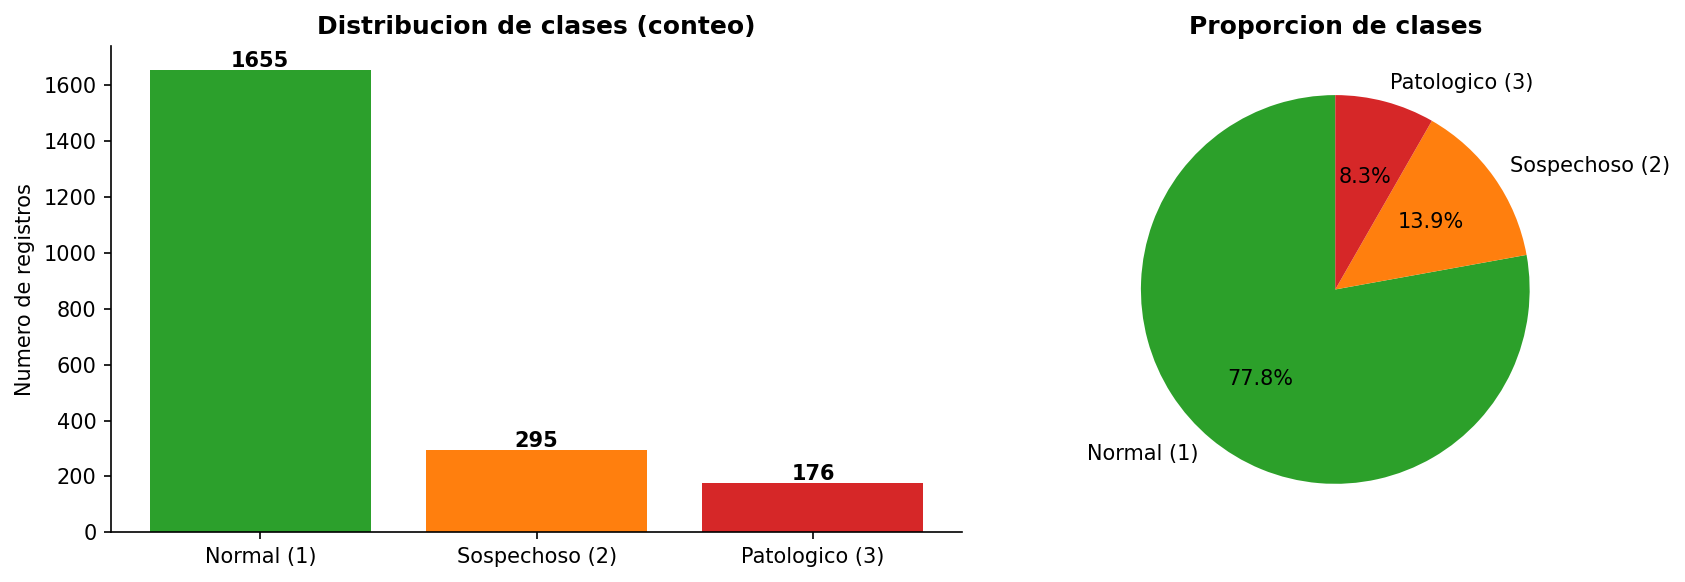
\includegraphics[width=0.9\textwidth]{fig_distribucion_clases.png}
  \caption{Distribución de clases en el dataset CTG. Izquierda: conteo absoluto. Derecha: proporción porcentual.}
  \label{fig:distribucion_clases}
\end{figure}

\subsection{Retos del dataset}

Identificamos cinco desafíos metodológicos con implicaciones directas sobre el preprocesamiento
y la elección de algoritmos:

\begin{enumerate}[label=\Alph*.]
  \item \textbf{Desbalance de clases.} El 78\,\% de los registros pertenecen a la clase Normal,
  lo que puede llevar a que los algoritmos basados en distancia absorban los casos de
  Sospechoso y Patológico al grupo mayoritario.
  \item \textbf{Heterogeneidad de escalas.} \texttt{baseline\_value} opera en el rango
  100--160 mientras que \texttt{accelerations} lo hace en 0.000--0.018. Sin estandarización,
  cualquier cálculo de distancia sobrepondera la primera variable.
  \item \textbf{Multicolinealidad.} \texttt{histogram\_mode}, \texttt{histogram\_mean} y
  \texttt{histogram\_median} son representaciones distintas de la misma señal cardíaca,
  con correlaciones típicamente superiores a 0.90 entre ellas.
  \item \textbf{Variables con baja varianza.} \texttt{severe\_decelerations} es prácticamente
  constante (5 registros con valor distinto de cero sobre 2{,}126).
  \item \textbf{Outliers.} \texttt{histogram\_variance} presenta valores extremos superiores
  a 120 mientras la mayoría se encuentra por debajo de 10.
\end{enumerate}

%%%%%%%%%%%%%%%%%%%%%%%%%%%%%%%%%%
\newpage
%%%%%%%%%%%%%%%%%%%%%%%%%%%%%%%%%%

%%%%%%%%%%%%%%%%%%%%%%%%%%%%%%%%%%
\section{Preprocesamiento}
%%%%%%%%%%%%%%%%%%%%%%%%%%%%%%%%%%

\subsection{Auditoría y limpieza}

Comenzamos verificando programáticamente la completitud del dataset. Se confirmó la ausencia
de valores nulos, valores centinela ($-999$) y cadenas vacías en las 22 columnas. Adicionalmente,
identificamos y eliminamos registros duplicados exactos para evitar sesgar los centroides de
K-Means hacia regiones sobrerepresentadas.

La consistencia de rangos clínicos se verificó para las variables con límites fisiológicamente
definidos (\texttt{baseline\_value} entre 50 y 200, porcentajes entre 0 y 100, \texttt{fetal\_health}
entre 1 y 3). No se encontraron registros fuera de rango.

\subsection{Tratamiento de outliers}

Empleamos el criterio del rango intercuartílico (IQR): todo valor por debajo de
$Q_1 - 1.5\cdot\text{IQR}$ o por encima de $Q_3 + 1.5\cdot\text{IQR}$ se consideró
candidato a outlier (Figura~\ref{fig:boxplots_outliers}). La decisión sobre su tratamiento
dependió del contexto clínico: los outliers asociados a casos Patológicos se conservaron
para no sesgar el análisis hacia los grupos mayoritarios.

\begin{figure}[H]
  \centering
  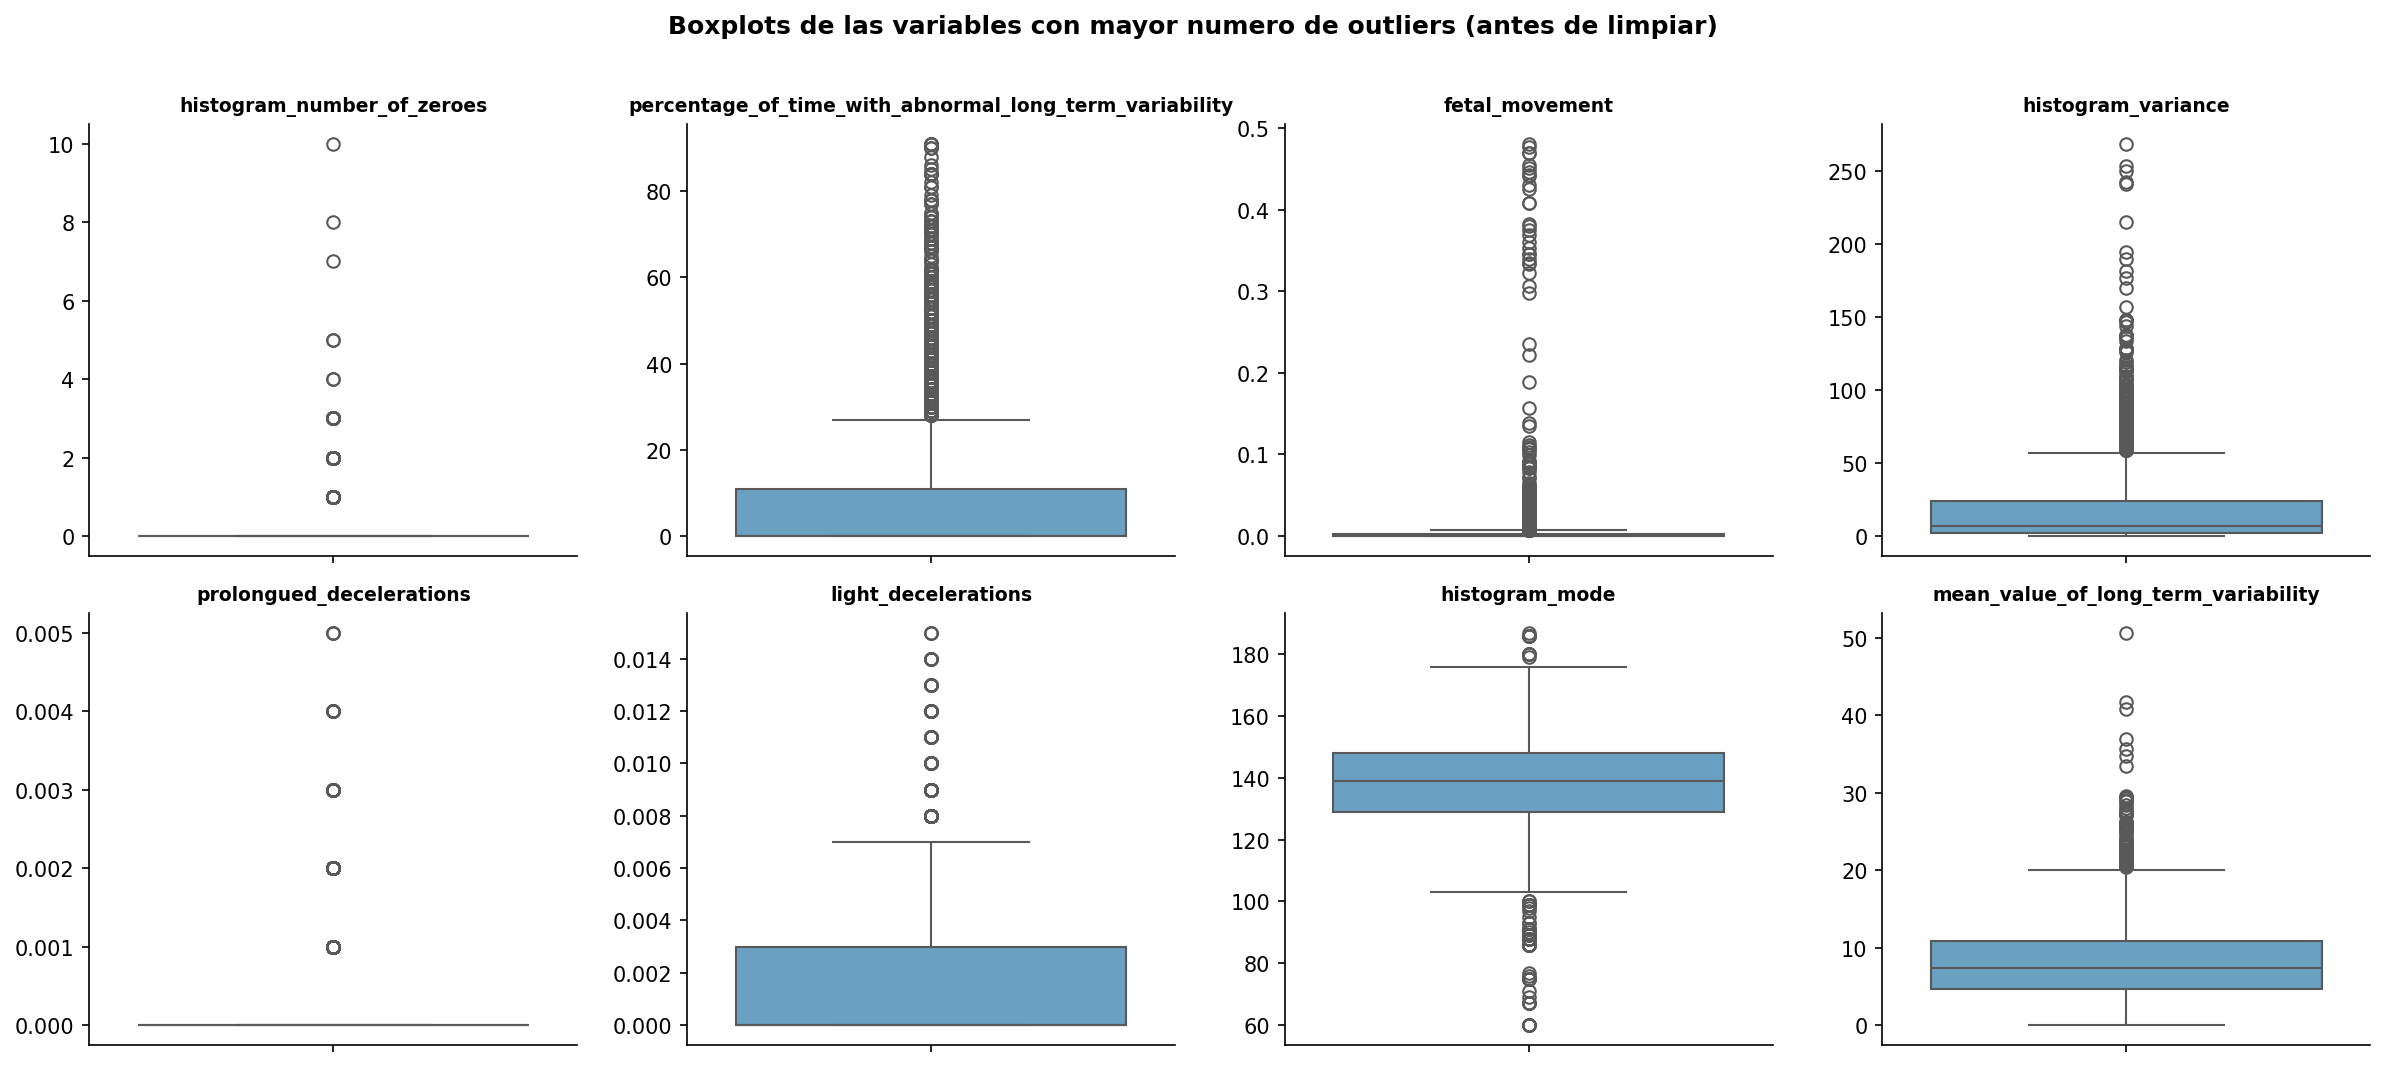
\includegraphics[width=0.95\textwidth]{fig_boxplots_outliers.png}
  \caption{Boxplots de las variables con mayor número de outliers. Las cajas comprimidas
           en cero de \texttt{prolongued\_decelerations} y \texttt{fetal\_movement}
           reflejan la infrecuencia clínica de esos eventos.}
  \label{fig:boxplots_outliers}
\end{figure}

Variables como \texttt{histogram\_number\_of\_zeroes}, \texttt{prolongued\_decelerations}
y \texttt{fetal\_movement} presentan la caja comprimida cerca de cero con outliers dispersos
hacia arriba, lo que es clínicamente esperable: las desaceleraciones prolongadas y los
movimientos fetales intensos son eventos poco frecuentes. Por contraste,
\texttt{percentage\_of\_time\_with\_abnormal\_long\_term\_variability} muestra una caja
más amplia con una concentración de outliers entre 70 y 95, lo que sugiere una
subpoblación con variabilidad anormal elevada. Las variables del histograma como
\texttt{histogram\_variance} presentan dispersión moderada con outliers en ambos extremos.
En todos los casos optamos por conservar estos valores extremos ya que representan
registros clínicos reales, aplicando en su lugar transformaciones logarítmicas para
reducir el efecto de las colas sin perder información.

\subsection{Análisis de correlaciones}

Construimos la matriz de correlación de Pearson para confirmar empíricamente la
multicolinealidad anticipada (Figura~\ref{fig:heatmap_corr}). Los pares con correlación
absoluta superior a 0.85 incluyen \texttt{histogram\_mode}, \texttt{histogram\_mean} y
\texttt{histogram\_median}, lo que justifica la reducción de dimensionalidad con PCA.

\begin{figure}[H]
  \centering
  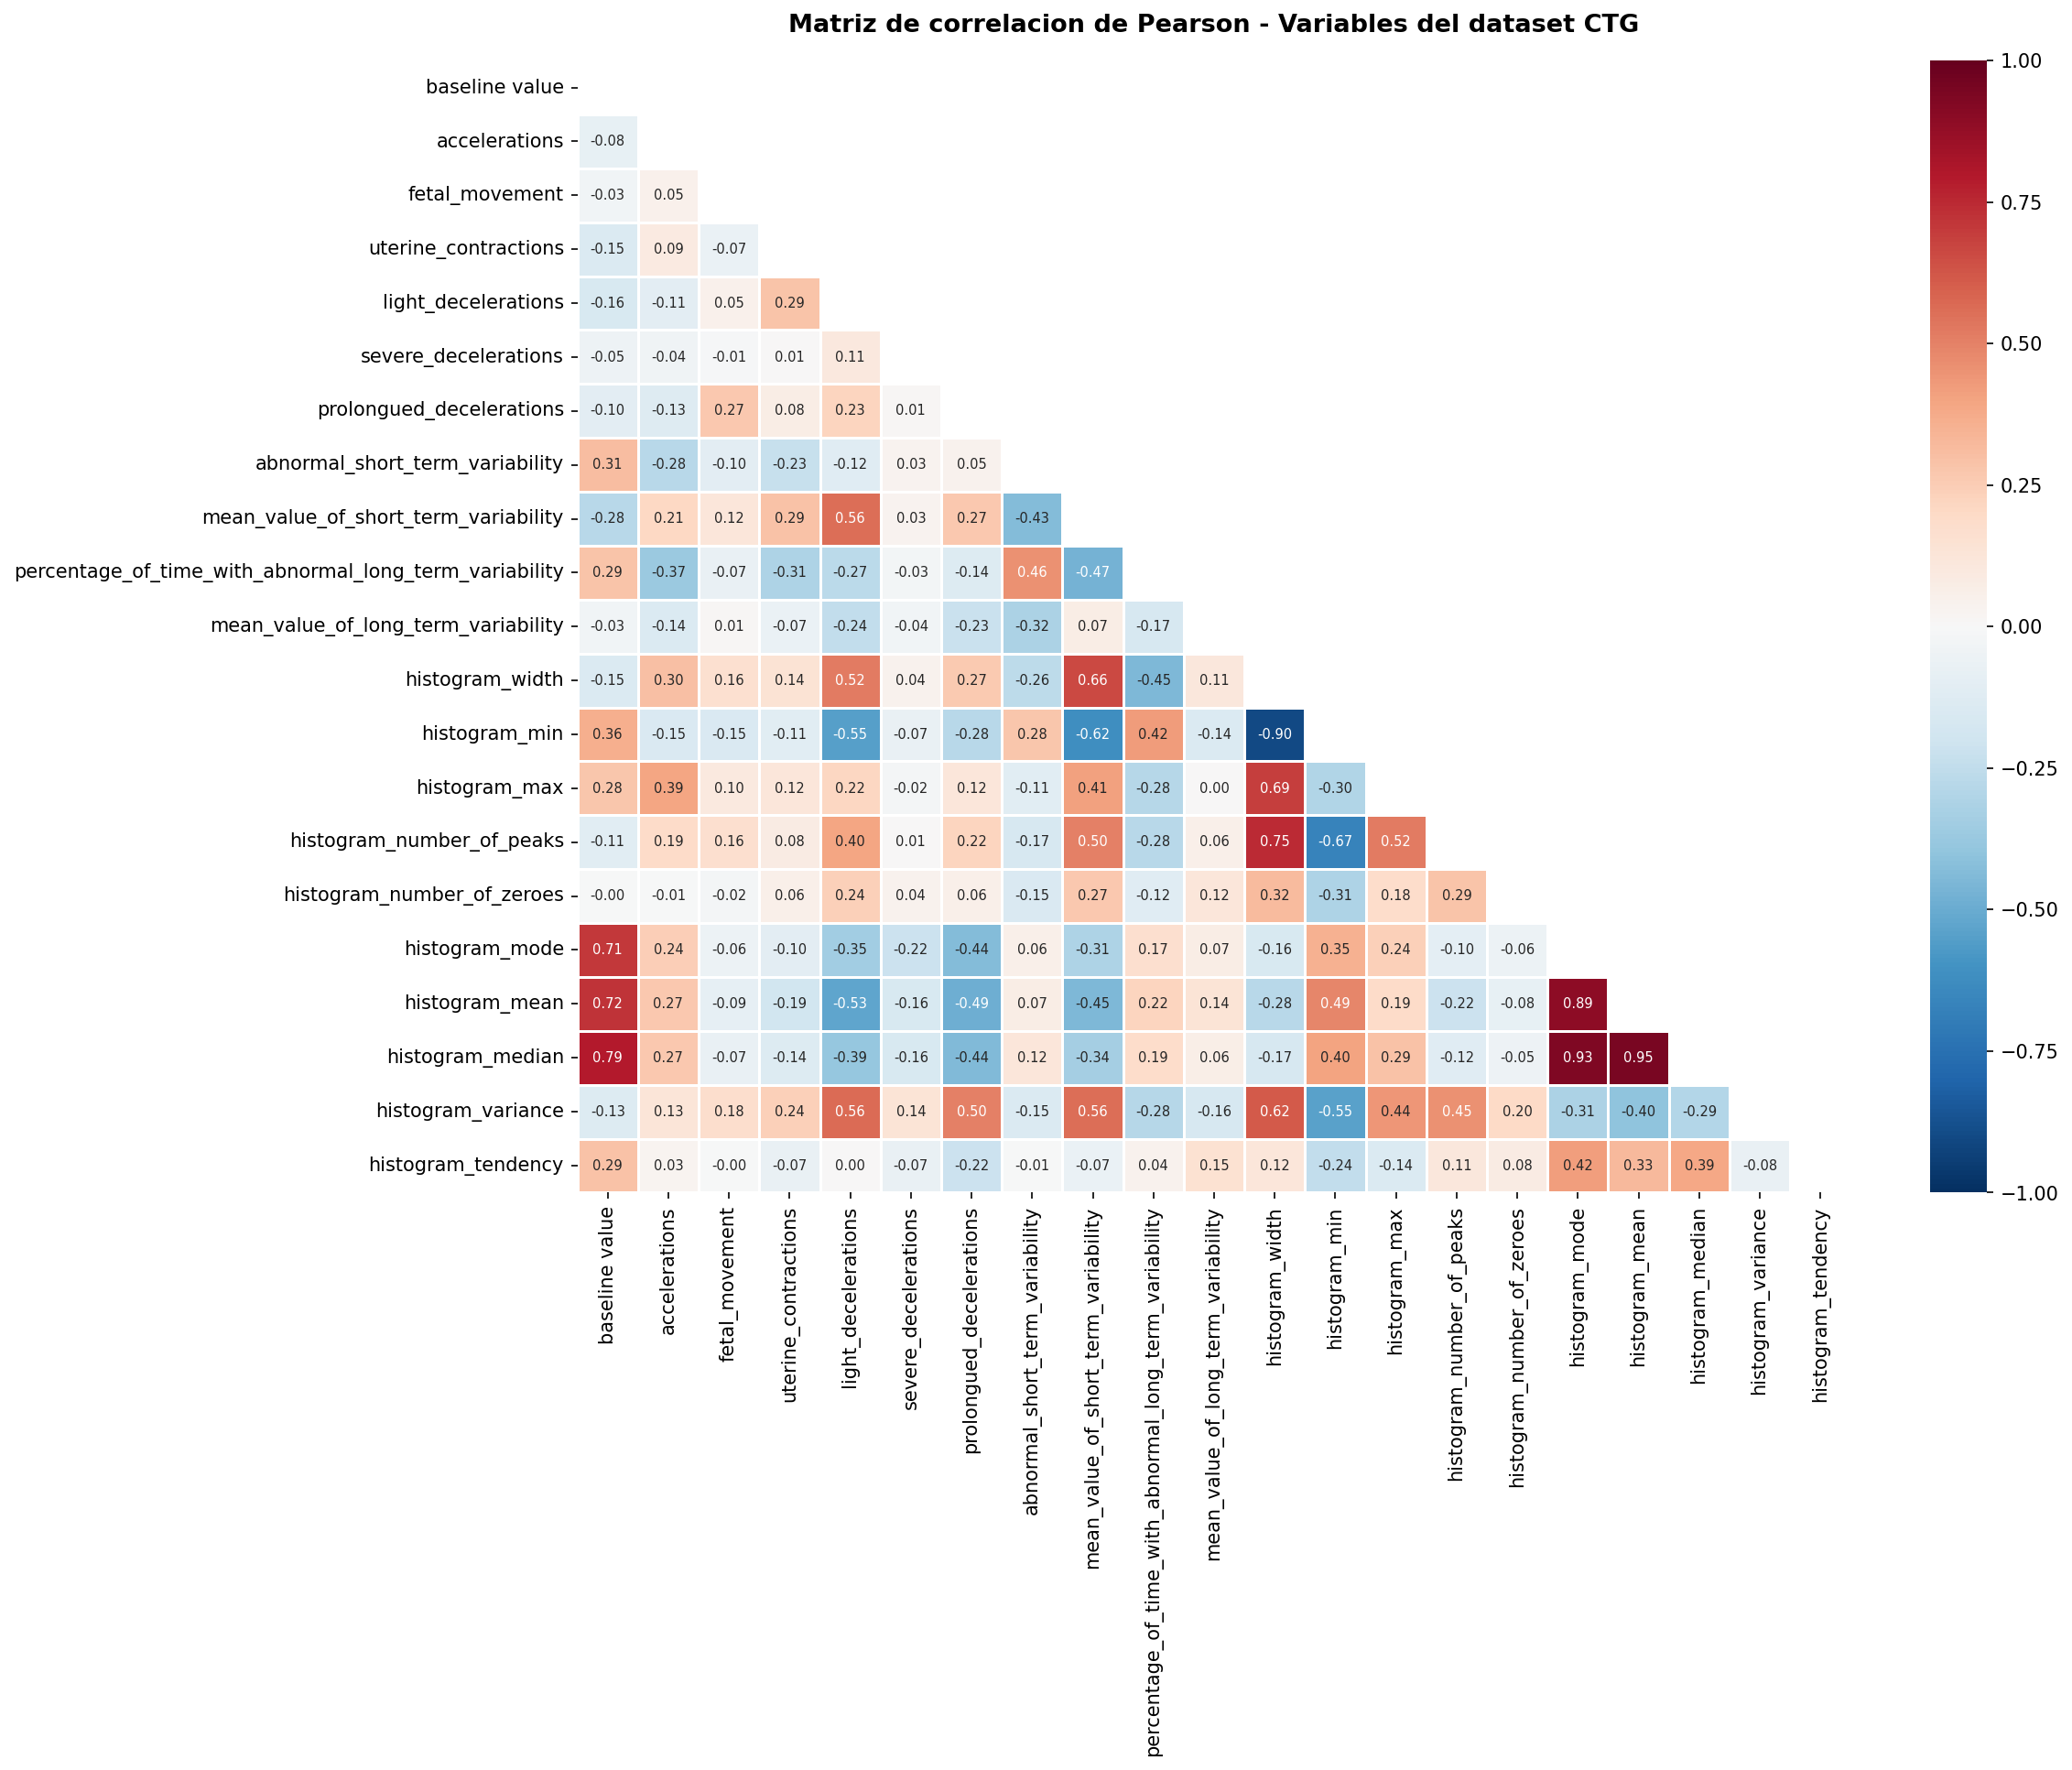
\includegraphics[width=0.88\textwidth]{fig_heatmap_correlaciones.png}
  \caption{Matriz de correlación de Pearson de las 21 variables de entrada. El bloque
           superior derecho concentra las correlaciones más altas entre variables del histograma.}
  \label{fig:heatmap_corr}
\end{figure}

El heatmap confirma la redundancia esperada entre las variables del histograma de FCF.
Los pares \texttt{histogram\_median}--\texttt{histogram\_mean} ($r=0.95$),
\texttt{histogram\_median}--\texttt{histogram\_mode} ($r=0.93$) y
\texttt{histogram\_mean}--\texttt{histogram\_mode} ($r=0.89$) presentan correlaciones muy
altas porque las tres son medidas de tendencia central de la misma distribución. De manera
similar, \texttt{histogram\_min} y \texttt{histogram\_max} muestran correlación negativa
fuerte ($r=-0.90$) con otras variables del histograma, ya que los extremos están
intrínsecamente ligados al ancho de la distribución. Las variables de eventos clínicos
(aceleraciones, contracciones, desaceleraciones) muestran correlaciones bajas entre sí,
lo que indica que aportan información complementaria y no redundante. Esta multicolinealidad
justifica el uso de PCA para reducir la dimensionalidad sin perder información relevante.

\subsection{Normalización y estandarización}

Dado que K-Means, DBSCAN y el clustering jerárquico operan sobre distancias euclidianas,
la diferencia de escalas es uno de los problemas más críticos. Aplicamos la siguiente
estrategia en dos pasos:

\begin{enumerate}
  \item \textbf{Transformación logarítmica} $\log(x+1)$ sobre las variables con distribución
  fuertemente asimétrica y alta esparsidad (\texttt{fetal\_movement},
  \texttt{prolongued\_decelerations}, \texttt{histogram\_variance}).
  \item \textbf{Estandarización Z-score} (media 0, desviación estándar 1) sobre la totalidad
  de las variables transformadas.
\end{enumerate}

La Figura~\ref{fig:distribuciones_post} muestra las distribuciones resultantes tras el
preprocesamiento completo.

\begin{figure}[H]
  \centering
  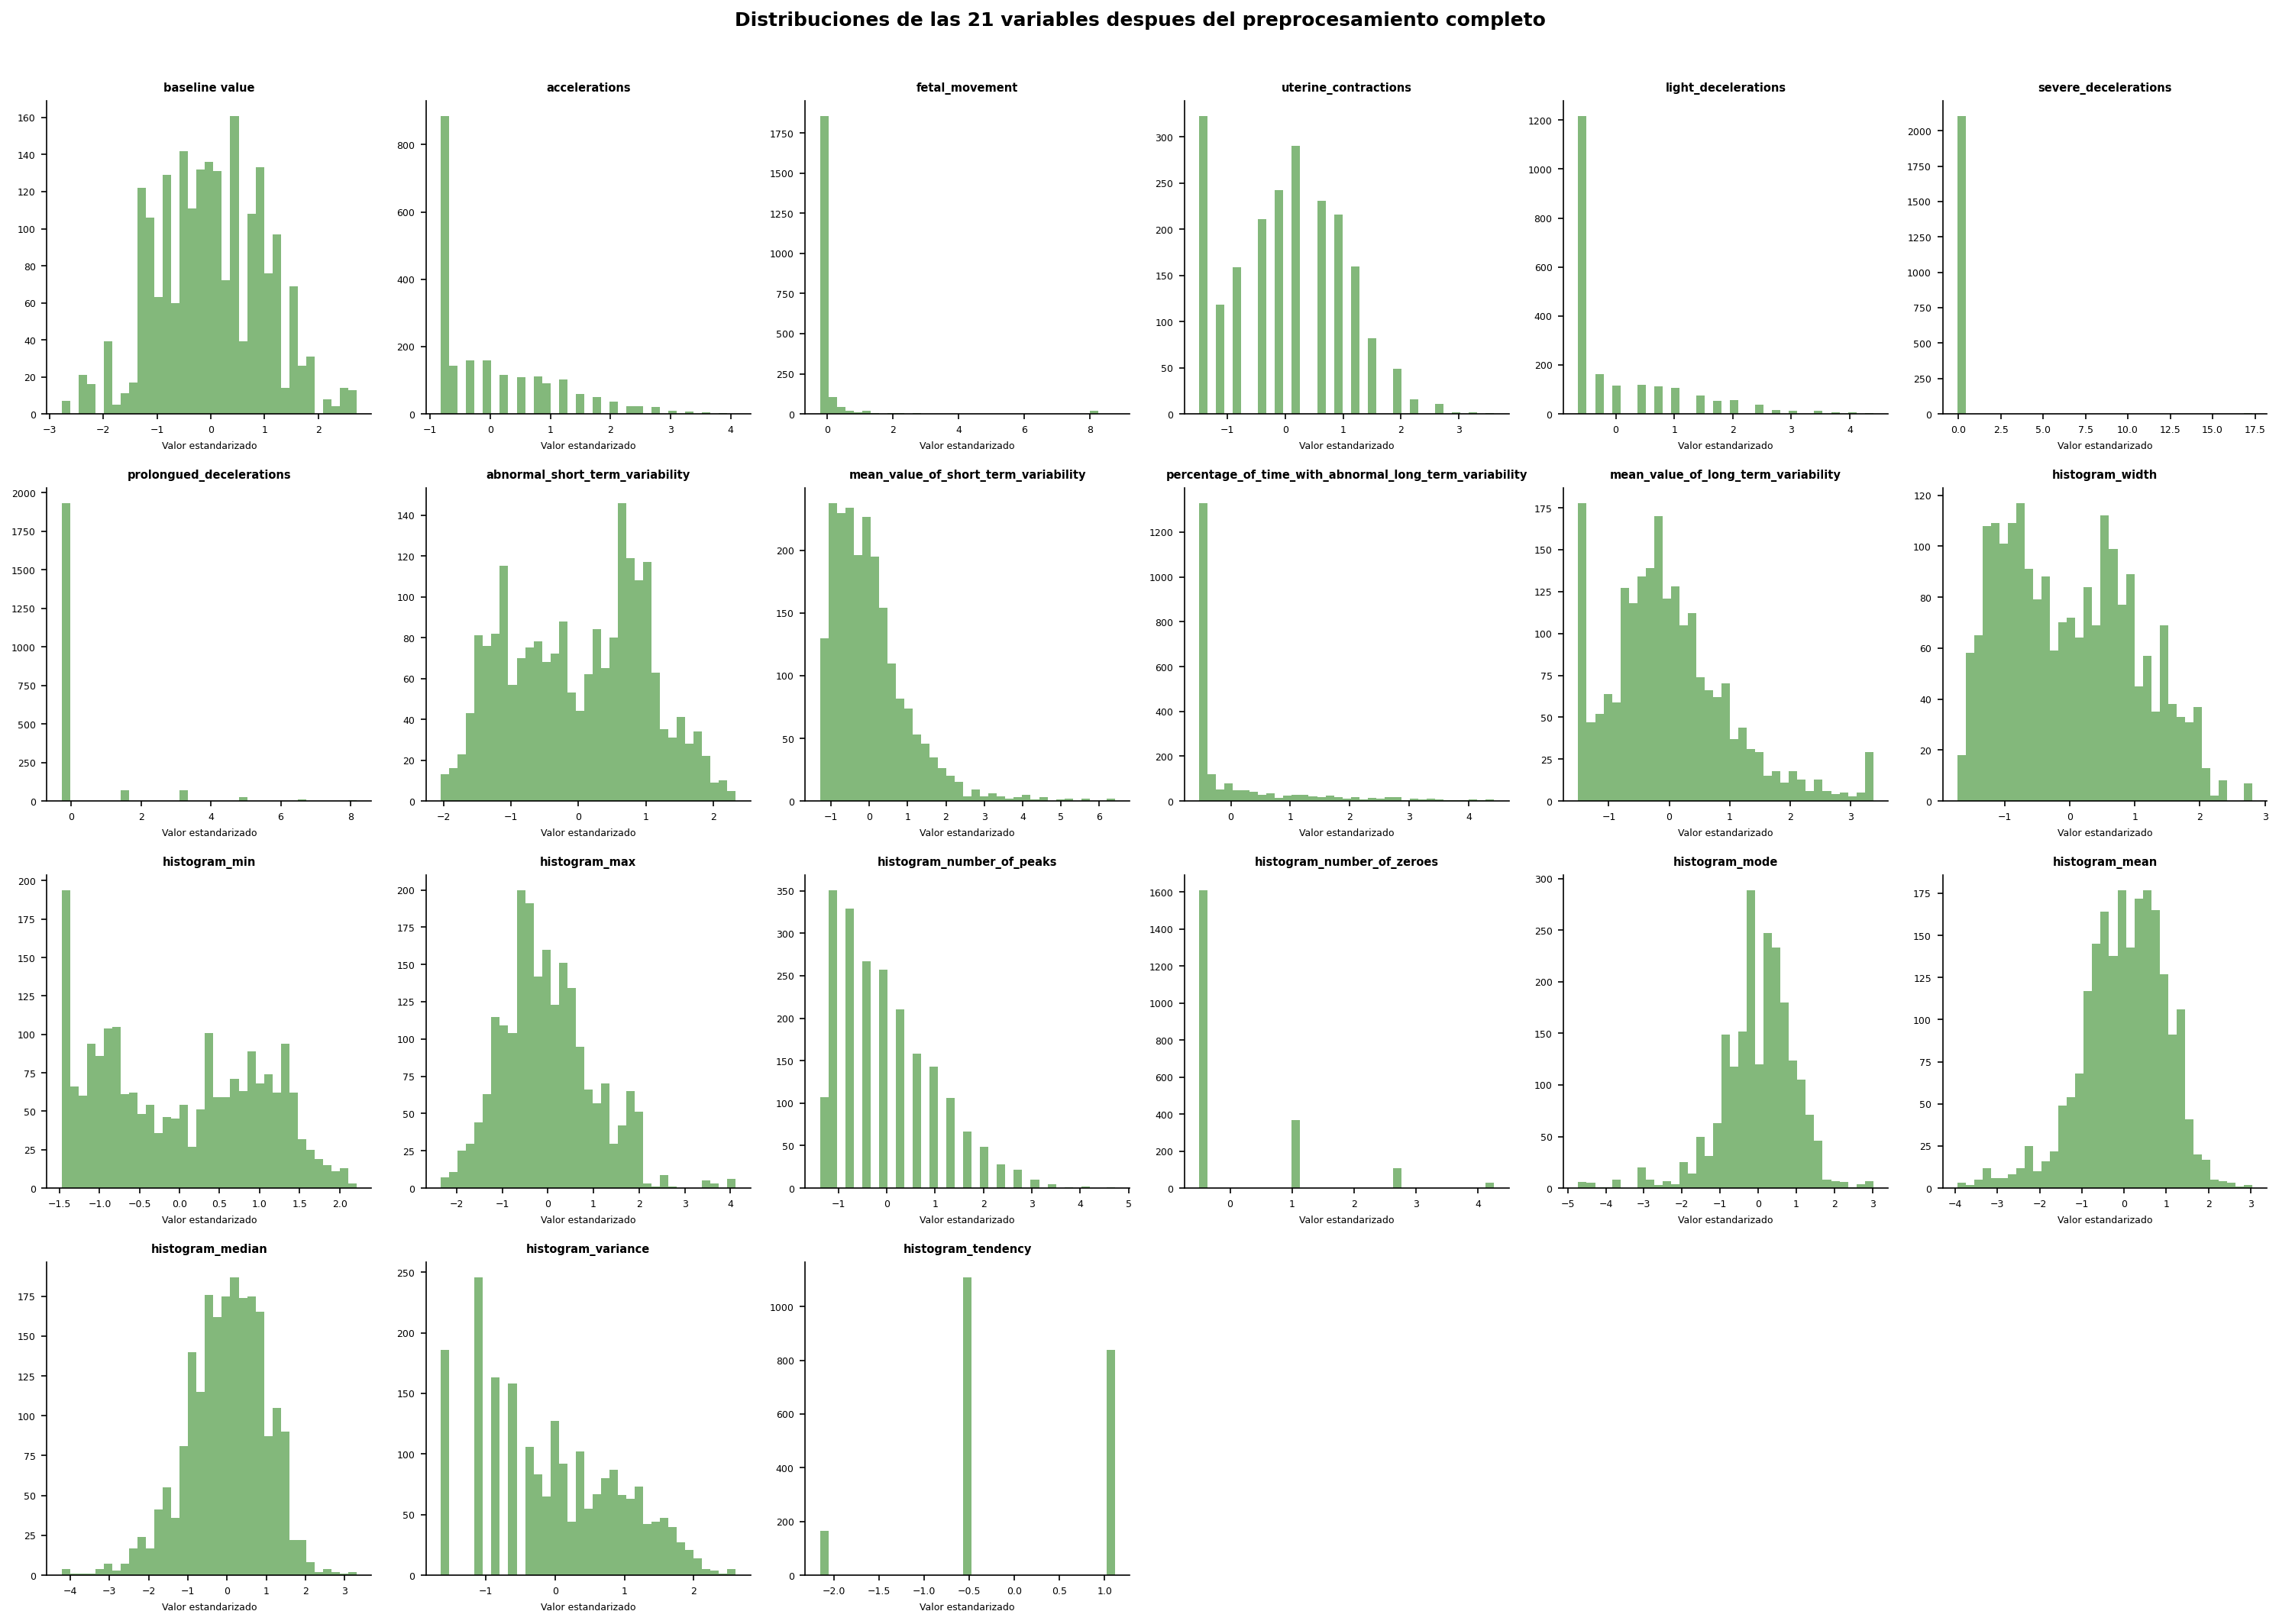
\includegraphics[width=0.95\textwidth]{fig_distribuciones_post_prep.png}
  \caption{Distribuciones de las 21 variables estandarizadas tras el preprocesamiento. Se
           distinguen tres grupos de comportamiento según la forma resultante de cada histograma.}
  \label{fig:distribuciones_post}
\end{figure}

La transformación logarítmica tuvo un efecto variable según la naturaleza de cada columna.
Para \texttt{histogram\_variance} y \texttt{light\_decelerations} la mejora es notable:
la distribución pasa de una cola larga hacia la derecha a una forma más extendida y
simétrica. Para \texttt{fetal\_movement}, \texttt{severe\_decelerations} y
\texttt{prolongued\_decelerations}, la concentración en cero persiste incluso tras la
transformación, lo que refleja que la mayoría de los registros genuinamente registran
ausencia de esos eventos clínicos. Tras la estandarización Z-score, los histogramas
verdes permiten distinguir tres tipos de comportamiento: variables con distribución
aproximadamente normal (\texttt{baseline\_value}, \texttt{histogram\_min},
\texttt{histogram\_mean}), variables con sesgo positivo moderado
(\texttt{accelerations}, \texttt{uterine\_contractions}), y variables con alta
concentración en un único valor que reflejan la infrecuencia intrínseca de ciertos
eventos clínicos. El dataset queda así sin valores faltantes, con outliers atenuados
y todas las variables en la misma escala.

\subsection{Reducción de dimensionalidad (PCA)}

Aplicamos PCA con umbral de varianza del 95\,\% para determinar el número mínimo de
componentes necesarios. Los algoritmos de clustering operaron tanto sobre el espacio
original estandarizado como sobre los componentes principales para comparar si la
reducción mejora la separabilidad.

\begin{figure}[H]
  \centering
  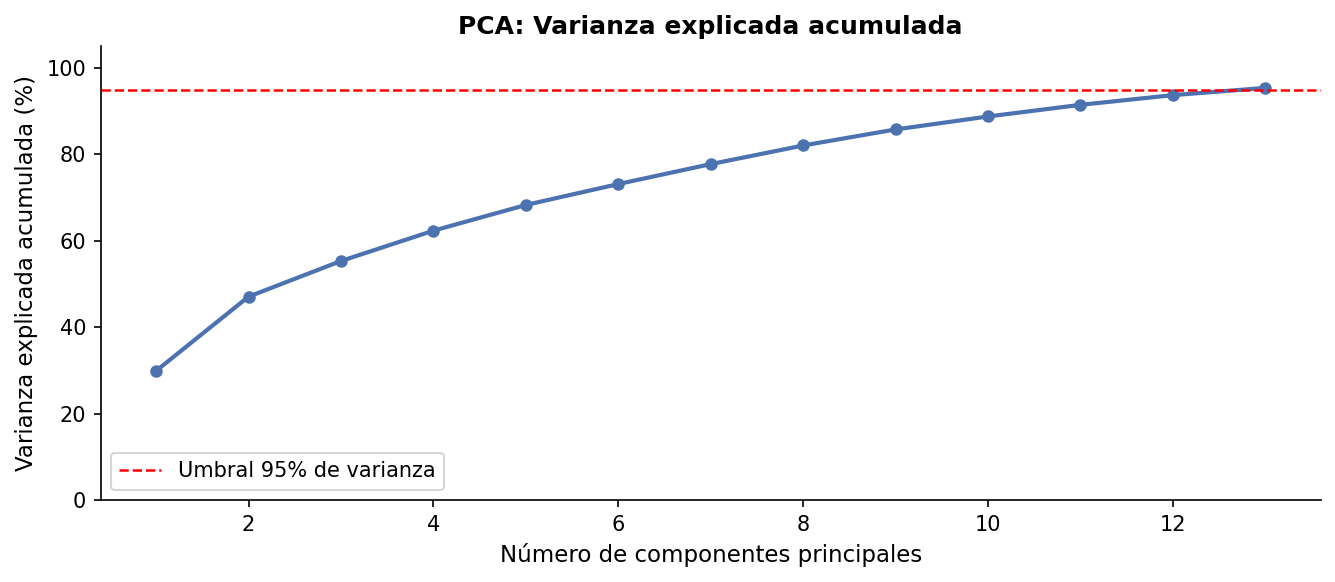
\includegraphics[width=0.75\textwidth]{fig_pca_varianza_explicada.png}
  \caption{Varianza explicada acumulada por componente principal. La línea roja marca el
           umbral del 95\,\%. Se requieren 13 componentes para alcanzarlo.}
  \label{fig:pca_varianza}
\end{figure}

La curva muestra que ningún componente domina de forma clara: el primero explica apenas
el 30\,\% y la curva crece de forma gradual y continua sin un codo pronunciado. Para
alcanzar el umbral del 95\,\% son necesarios 13 componentes sobre los 21 originales,
indicando que la información está distribuida de manera relativamente uniforme entre las
variables. Esta ausencia de un quiebre abrupto anticipa que los algoritmos operarán en
un espacio intrínsecamente de alta dimensión. Para las visualizaciones utilizamos los dos
primeros componentes (PC1 y PC2, aproximadamente el 47\,\% acumulado) como proyección
exploratoria, sin pretender que representen la geometría completa del espacio.


%%%%%%%%%%%%%%%%%%%%%%%%%%%%%%%%%%
\newpage
%%%%%%%%%%%%%%%%%%%%%%%%%%%%%%%%%%

%%%%%%%%%%%%%%%%%%%%%%%%%%%%%%%%%% 
\section{Modelos de Clustering}
%%%%%%%%%%%%%%%%%%%%%%%%%%%%%%%%%%

La selección de algoritmos no es arbitraria: cada método hace supuestos distintos sobre la
forma, densidad y distribución de los datos. Implementamos tres paradigmas complementarios
que cubren el espacio de estrategias de agrupamiento más relevantes para este problema.

\subsection{K-Means++ (clustering particional)}

K-Means++ extiende el K-Means clásico mejorando el procedimiento de inicialización:
los centroides iniciales se eligen de forma que estén lo más separados posible entre sí,
evitando convergencia a mínimos locales subóptimos. Dado un número $k$ de clusters, el
algoritmo minimiza iterativamente la inercia (suma de distancias cuadráticas de cada punto
a su centroide más cercano):

\[
  \mathcal{J} = \sum_{i=1}^{N} \left\| \mathbf{x}_i - \boldsymbol{\mu}_{c(i)} \right\|^2
\]

Su aplicación en este dataset se justifica por tres razones: conocemos de antemano que el
problema tiene tres categorías clínicas (valor de $k$ biológicamente motivado), es
computacionalmente eficiente con 2{,}126 registros y 21 variables, y sus centroides en el
espacio estandarizado pueden interpretarse clínicamente. Su limitación principal es que
asume clusters de forma esférica y tamaño similar, lo que puede no reflejar la geometría real.

\paragraph{Selección de $k$.} El método del codo y la curva de Silhouette promedio para
$k \in \{2,\ldots,8\}$ se muestran en la Figura~\ref{fig:codo_kmeans}.

\begin{figure}[H]
  \centering
  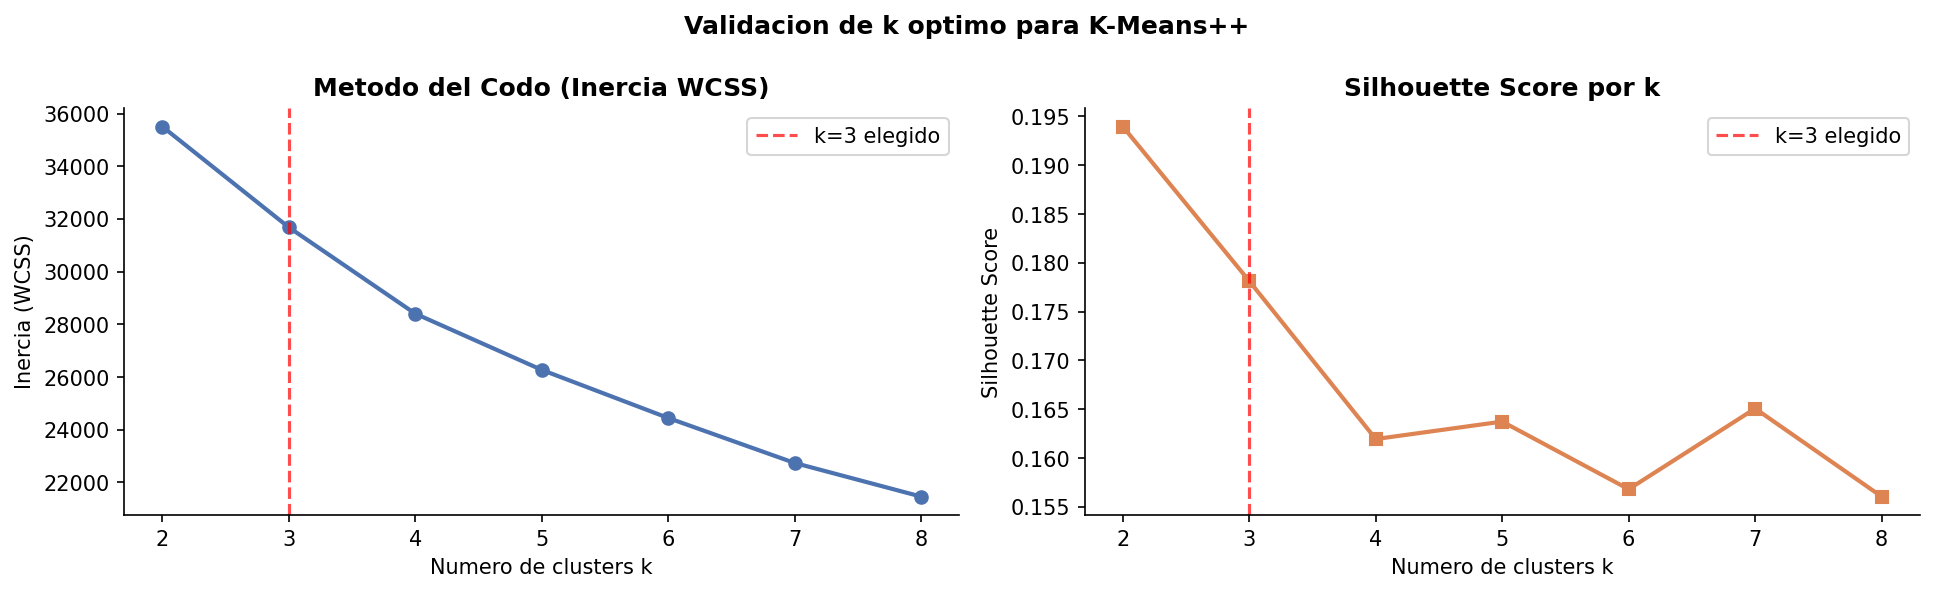
\includegraphics[width=0.88\textwidth]{fig_codo_kmeans.png}
  \caption{Método del codo (inercia WCSS) y Silhouette Score promedio para K-Means++
           con $k=2,\ldots,8$. La línea roja indica $k=3$.}
  \label{fig:codo_kmeans}
\end{figure}

La inercia WCSS decrece de forma continua y sin un quiebre pronunciado entre $k=2$ y
$k=8$, lo que refleja la naturaleza gradual de las fronteras entre los estados de salud
fetal. La curva de Silhouette muestra su valor máximo en $k=2$ (0.194) y cae a 0.179
en $k=3$, manteniéndose por debajo de ese nivel para $k\geq4$. Aunque el Silhouette
sugeriría $k=2$ de forma puramente geométrica, la existencia de tres categorías clínicas
con sustento médico claro (Normal, Sospechoso, Patológico) motiva la elección de $k=3$.
Ambas curvas coinciden en que valores mayores no aportan separabilidad adicional.

\subsection{DBSCAN (clustering basado en densidad)}

DBSCAN identifica regiones del espacio donde los puntos se encuentran densamente agrupados
y declara como ruido (\textit{noise}) a los puntos que no pertenecen a ninguna región densa.
Requiere dos hiperparámetros: $\varepsilon$ (radio de vecindad) y \texttt{min\_samples}
(mínimo de puntos para constituir un núcleo). Su elección responde directamente a uno de
los retos del dataset: la presencia de variables con distribuciones extremadamente asimétricas
y esparsas. DBSCAN es el único algoritmo del conjunto capaz de tratar registros extremos de
forma explícita, clasificándolos como ruido en lugar de absorberlos al grupo más cercano.

\paragraph{Calibración de hiperparámetros.} Para determinar $\varepsilon$ calculamos la
distancia al vecino $k=41$ ($= 2 \cdot 21 - 1$) para cada punto del dataset, ordenando
los resultados de mayor a menor (Figura~\ref{fig:kdist_dbscan}). El percentil del 2\,\%
de puntos más alejados sugiere un codo en $\varepsilon_0 \approx 6.3$. Sobre ese valor
se realizó un grid search en la rejilla $\varepsilon \in [0.5\varepsilon_0,\, 2\varepsilon_0]$
y \texttt{min\_samples} $\in \{5, 10, 15, 20, 30\}$, resultando en la configuración final
$\varepsilon = 3.155$ y \texttt{min\_samples} $= 5$.

\begin{figure}[H]
  \centering
  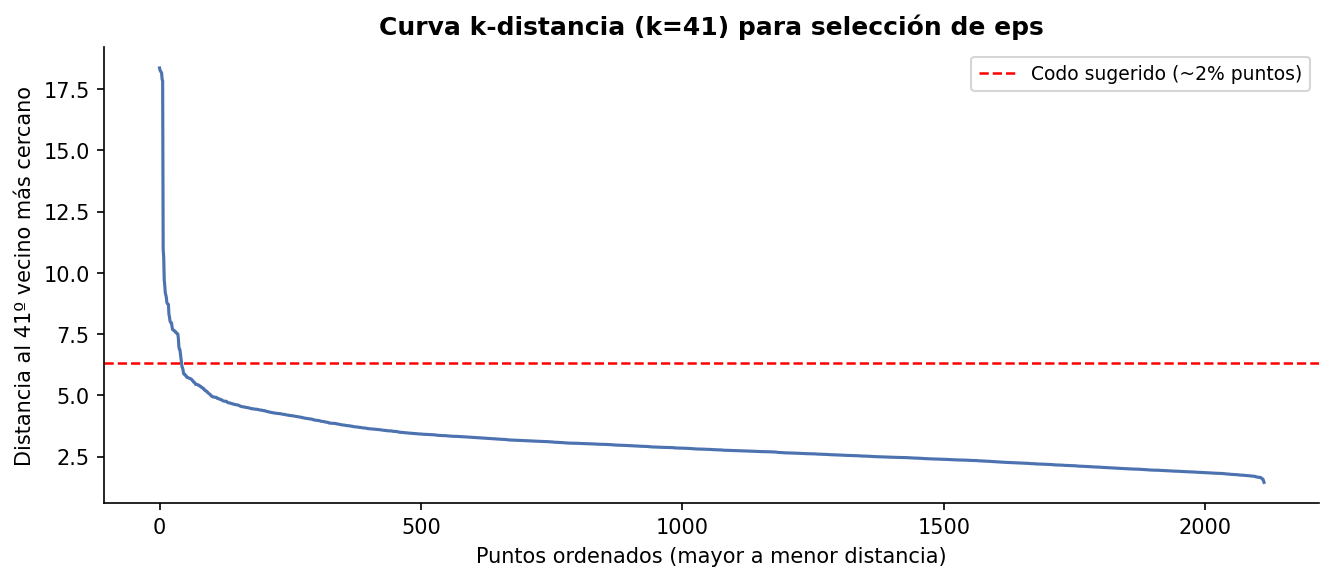
\includegraphics[width=0.75\textwidth]{fig_dbscan_kdist.png}
  \caption{Curva de distancias al vecino 41 ($k=41$) para calibrar $\varepsilon$ en DBSCAN.
           La curva cae abruptamente en los primeros ${\sim}100$ puntos (de 18 a 6) y luego
           decrece de forma suave. La línea roja discontinua marca el codo sugerido
           en $\varepsilon_0 \approx 6.3$ (percentil 2\,\% de puntos más alejados).}
  \label{fig:kdist_dbscan}
\end{figure}

La caída pronunciada en los primeros 100 puntos corresponde a los outliers del dataset
(registros con vecinos muy lejanos), mientras que la cola suave desde el punto 200 hasta
el 2126 indica que la gran mayoría de los registros se encuentran en regiones de densidad
relativamente uniforme. El codo en ${\sim}6.3$ marca la frontera entre la zona de ruido
y la zona de alta densidad, aunque el grid search final seleccionó $\varepsilon = 3.155$,
valor más conservador que fuerza una densidad mínima más estricta.

\subsection{Gaussian Mixture Models (modelo probabilístico)}

Los Modelos de Mezcla Gaussiana (GMM) estiman la probabilidad de que cada observación
pertenezca a cada uno de los $k$ componentes gaussianos mediante el algoritmo
Expectation-Maximization (EM). La ventaja más relevante para un dominio médico es la
\textbf{salida probabilística}: en lugar de asignar un feto al cluster 2, el modelo indica
que ese registro tiene, por ejemplo, un 65\,\% de probabilidad de corresponder al grupo
Sospechoso y un 35\,\% al Patológico. Esta ambigüedad cuantificada es clínicamente más
honesta en los casos límite donde la transición entre estados no es abrupta.

La flexibilidad de la matriz de covarianza permite clusters de forma elíptica (más realista
en un espacio de alta dimensión donde las variables no son independientes) y la selección
del número óptimo de componentes se apoya en los criterios BIC y AIC
(Figura~\ref{fig:bic_aic_gmm}).

\begin{figure}[H]
  \centering
  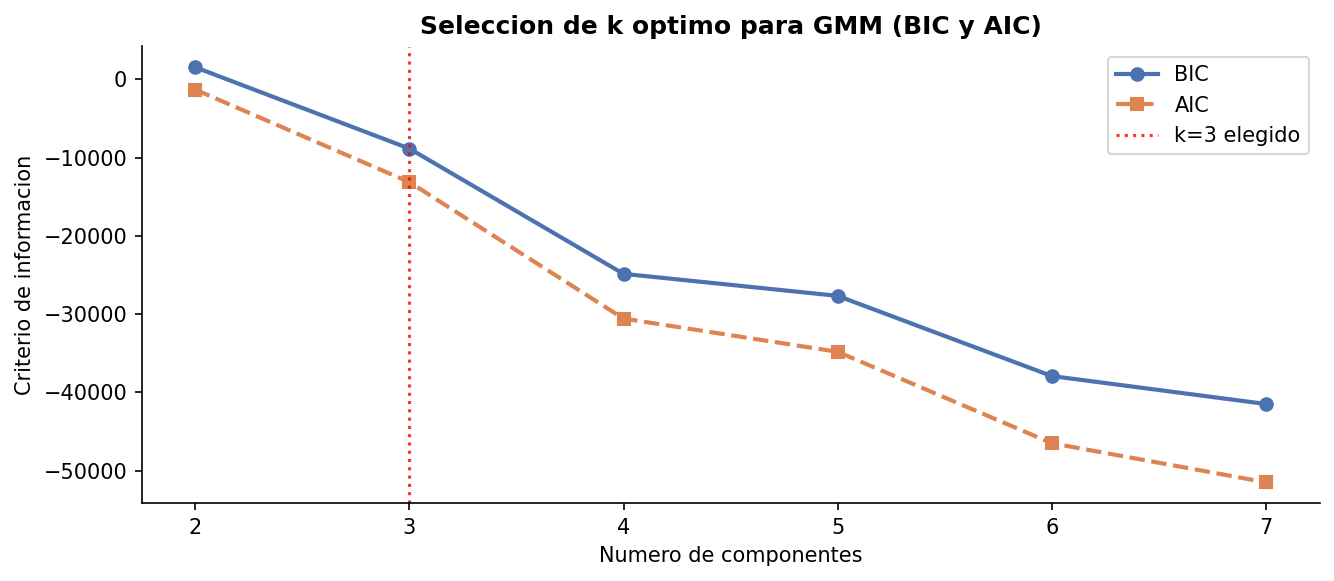
\includegraphics[width=0.72\textwidth]{fig_bic_aic_gmm.png}
  \caption{BIC y AIC para GMM con $k=2,\ldots,7$ componentes. Ambos criterios decrecen
           continuamente; la línea roja punteada marca $k=3$ elegido por motivación clínica.}
  \label{fig:bic_aic_gmm}
\end{figure}

A diferencia del caso ideal en que el BIC presenta un mínimo claro, aquí ambos criterios
decrecen de forma continua desde $k=2$ hasta $k=7$: el BIC pasa de valores cercanos a
cero en $k=2$ hasta aproximadamente $-42{,}000$ en $k=7$, mientras que el AIC desciende
de manera aún más pronunciada. Esto indica que, desde la perspectiva puramente estadística,
el modelo siempre mejora su ajuste al añadir más componentes. La elección de $k=3$
no está respaldada por un mínimo del BIC sino por la estructura clínica del problema
(tres estados de salud fetal reconocidos médicamente) y por la necesidad de mantener
una partición interpretable. Este resultado refuerza la idea de que el dataset no presenta
una separación gaussiana nítida en tres grupos, sino una estructura continua cuya
discretización en tres categorías es una convención diagnóstica más que una propiedad
geométrica intrínseca.

\subsection{Tabla comparativa de algoritmos}

\begin{table}[H]
\centering
\caption{Comparativa de los tres algoritmos de clustering implementados.}
\label{tab:comparativa_algos}
\footnotesize
\begin{tabular}{p{2.8cm}p{3.0cm}p{3.0cm}p{3.0cm}}
\toprule
\rowcolor{headbg}
\textbf{Criterio} & \textbf{K-Means++} & \textbf{DBSCAN} & \textbf{GMM} \\
\midrule
Paradigma             & Distancia (euclidiana) & Densidad local & Probabilístico (gaussiano) \\
Forma de clusters     & Esférica, convexa & Arbitraria, irregular & Elíptica (covarianza flexible) \\
Requiere $k$ inicial  & Sí ($k=3$) & No & Sí ($k=3$) \\
Manejo de outliers    & Los absorbe al centroide & Los etiqueta como ruido & Les asigna baja probabilidad \\
Salida del modelo     & Etiqueta dura $(0,1,2)$ & Etiqueta dura + ruido $(-1)$ & Probabilidad por cluster \\
Ventaja clave         & Línea base interpretable & Identifica casos raros & Incertidumbre por feto \\
\bottomrule
\end{tabular}
\end{table}

%%%%%%%%%%%%%%%%%%%%%%%%%%%%%%%%%%
\section{Métricas de Evaluación}
%%%%%%%%%%%%%%%%%%%%%%%%%%%%%%%%%%

Evaluamos la calidad del clustering en dos niveles complementarios: métricas internas
(coherencia geométrica sin usar etiquetas) y métricas externas (comparación con la
clasificación clínica de referencia).

\subsection{Métricas internas}

\textbf{Silhouette Score} $[-1, 1]$. Para cada observación mide la diferencia entre su
distancia media al propio cluster y al cluster vecino más cercano, normalizada por el
máximo de ambas. Un valor próximo a 1 indica buena asignación; cercano a 0, punto en la
frontera; negativo, posible mala asignación. Reportamos tanto el promedio global como los
diagramas de silueta individuales.

\textbf{Davies-Bouldin Index} $[0, +\infty)$. Para cada cluster calcula la ratio entre su
dispersión interna y su distancia al cluster más similar. El valor global es el promedio de
esas ratios; valores menores indican clusters simultáneamente compactos y bien separados.

\textbf{Calinski-Harabász Index} $[0, +\infty)$. Evalúa la relación entre la varianza
entre clusters y la varianza dentro de los clusters, ponderada por el número de observaciones
y grupos. Valores mayores indican mejor definición de la partición.

\subsection{Métricas externas}

Dado que el dataset incluye la etiqueta \texttt{fetal\_health}, disponemos de una referencia
externa de alta calidad para cuantificar en qué medida los grupos descubiertos coinciden
con la clasificación clínica.

\textbf{Adjusted Rand Index (ARI)} $(-1, 1]$. Mide la proporción de pares de observaciones
con el mismo tratamiento en ambas particiones, corregida por azar. Un ARI de 1 indica
concordancia perfecta; 0 equivale a asignación aleatoria.

\textbf{Normalized Mutual Information (NMI)} $[0, 1]$. Captura la información compartida
entre la partición generada y las etiquetas reales, normalizada para eliminar el sesgo por
número de clusters. Complementa al ARI al capturar dependencias estadísticas más generales.

\begin{table}[H]
\centering
\caption{Resumen de métricas de evaluación utilizadas.}
\label{tab:metricas}
\footnotesize
\begin{tabular}{llll}
\toprule
\rowcolor{headbg}
\textbf{Métrica} & \textbf{Tipo} & \textbf{Rango óptimo} & \textbf{Qué mide} \\
\midrule
Silhouette Score        & Interna  & Cercano a $+1$   & Cohesión interna y separación entre clusters \\
Davies-Bouldin Index    & Interna  & Mínimo posible   & Similitud promedio entre clusters adyacentes \\
Calinski-Harabász Index & Interna  & Máximo posible   & Relación varianza inter/intra cluster \\
ARI                     & Externa  & Cercano a $+1$   & Concordancia con etiquetas clínicas (correg. azar) \\
NMI                     & Externa  & Cercano a $1$    & Información compartida con diagnóstico real \\
\bottomrule
\end{tabular}
\end{table}

%%%%%%%%%%%%%%%%%%%%%%%%%%%%%%%%%%
\section{Resultados de Clustering}
%%%%%%%%%%%%%%%%%%%%%%%%%%%%%%%%%%

\subsection{K-Means++}

Entrenamos K-Means++ con $k=3$, \texttt{init='k-means++'}, \texttt{n\_init=20} y
\texttt{random\_state=42}. Las métricas internas obtenidas se muestran en la
Tabla~\ref{tab:metricas_clustering}.

La Figura~\ref{fig:kmeans_pca} muestra los clusters encontrados proyectados sobre los
dos primeros componentes principales, junto con la distribución de etiquetas clínicas
reales para comparación directa.

\begin{figure}[H]
  \centering
  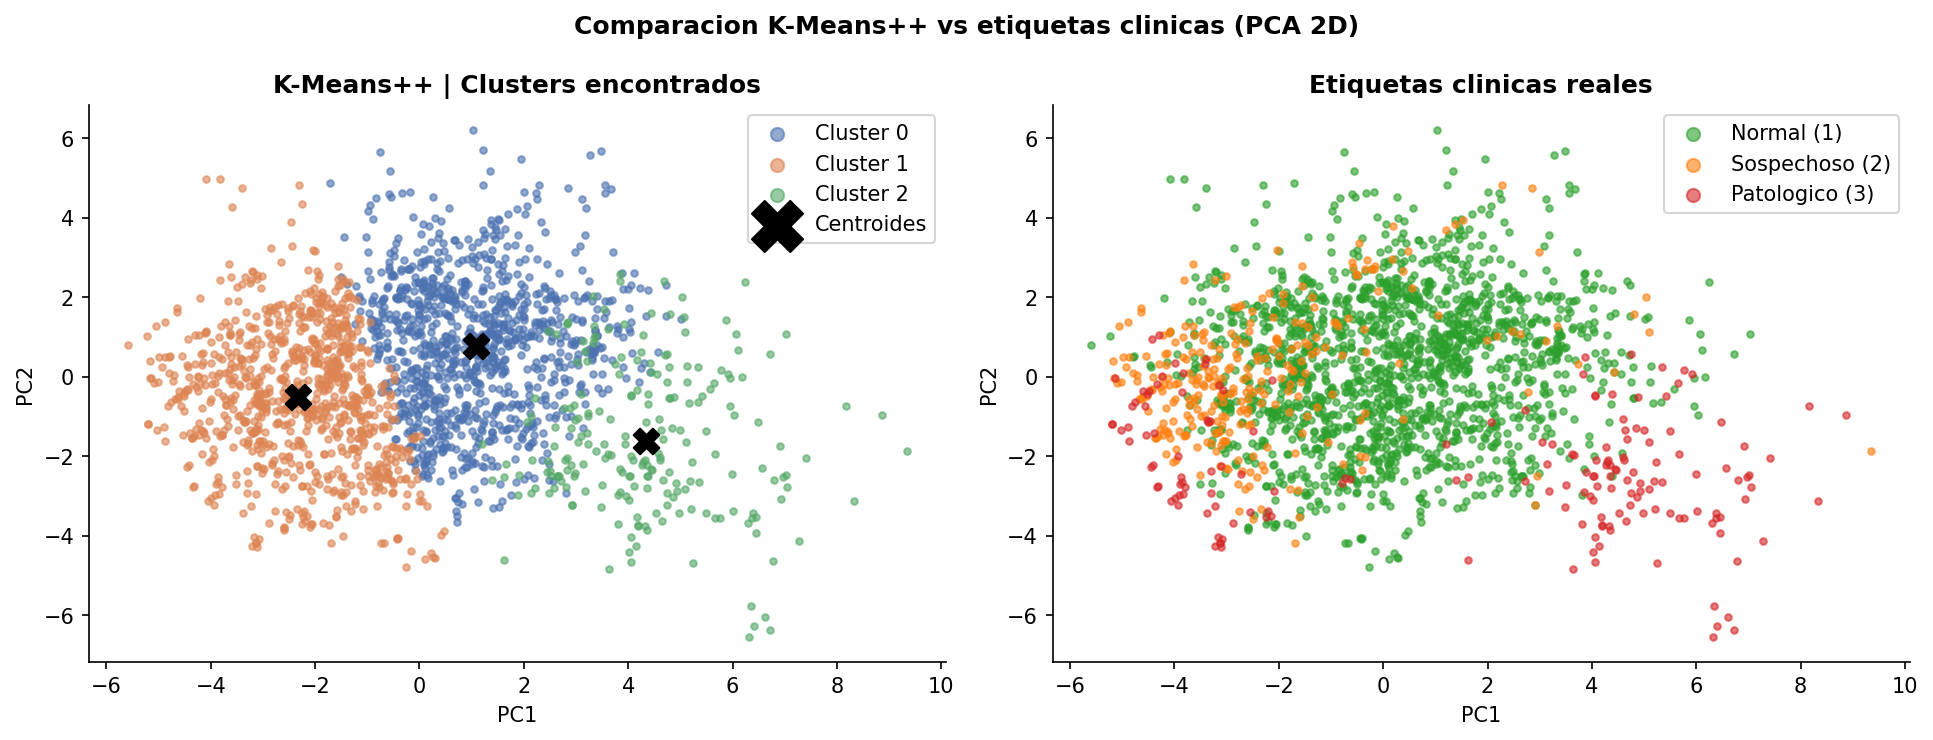
\includegraphics[width=0.88\textwidth]{fig_kmeans_pca2d.png}
  \caption{K-Means++ ($k=3$) en PCA 2D. Izquierda: clusters encontrados con centroides
           marcados (X). Derecha: etiquetas clínicas reales.}
  \label{fig:kmeans_pca}
\end{figure}

La comparación entre los dos paneles revela que K-Means++ logra separar una región
compacta hacia la derecha del espacio PCA (Cluster 2, $n=216$, verde) que corresponde
razonablemente con los casos Patológicos y parte de los Sospechosos. Sin embargo, los
Clusters 0 ($n=1{,}017$) y 1 ($n=880$) se solapan considerablemente en el espacio PCA,
lo que refleja que la frontera entre los estados Normal y Sospechoso no es geométricamente
nítida en las dos dimensiones de visualización. Este solapamiento es esperable dado que
PC1 y PC2 capturan solo el 47\,\% de la varianza total.

El diagrama de silueta individual (Figura~\ref{fig:silhouette_kmeans}) cuantifica la
cohesión interna de cada cluster.

\begin{figure}[H]
  \centering
  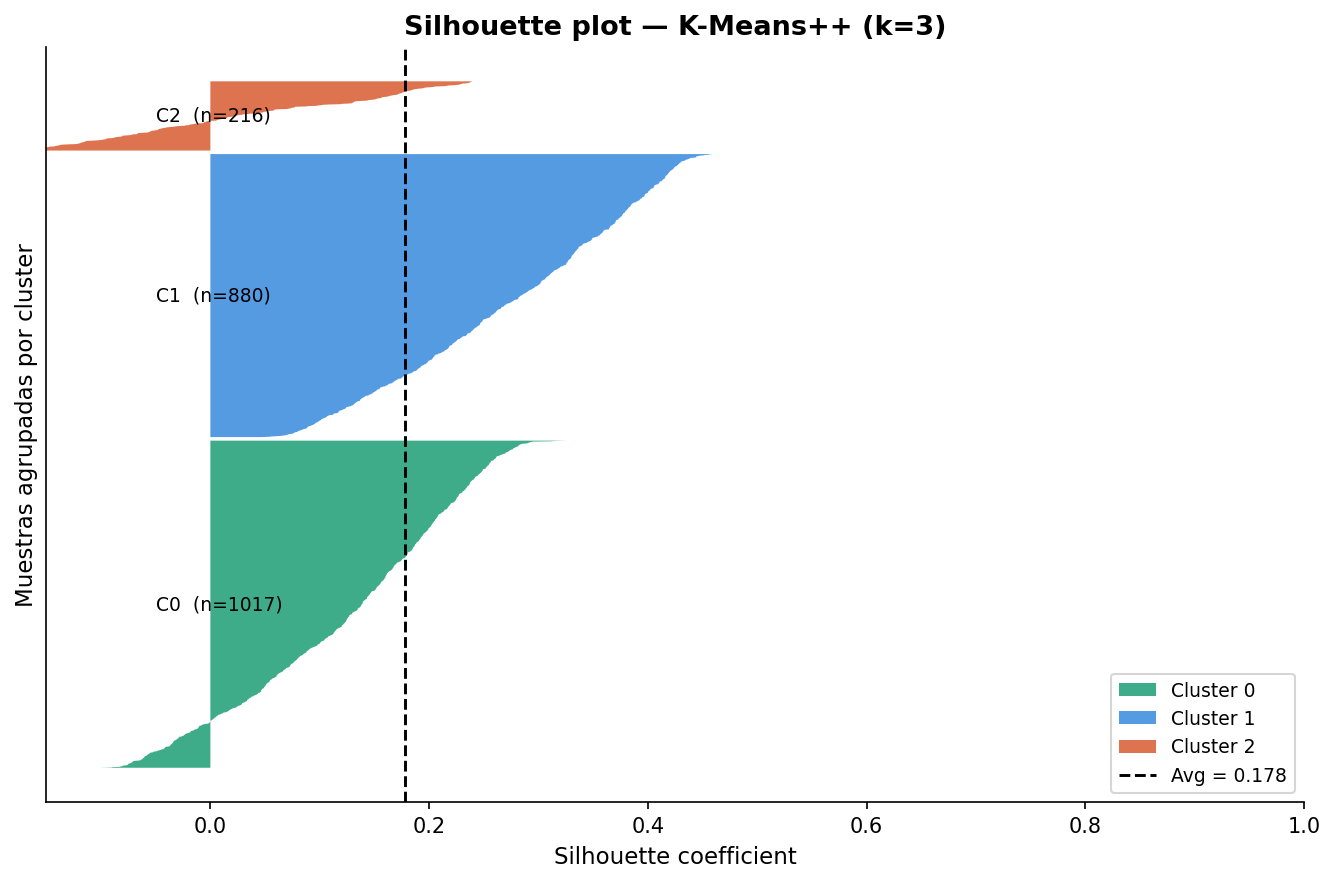
\includegraphics[width=0.70\textwidth]{fig_silhouette_kmeans.png}
  \caption{Silhouette plot para K-Means++ ($k=3$). Cada barra representa un registro;
           la línea discontinua indica el promedio global (\textit{Avg} = 0.178).}
  \label{fig:silhouette_kmeans}
\end{figure}

El Silhouette Score promedio de 0.178 confirma que la separación entre clusters es
modesta. El Cluster 2 ($n=216$) presenta los coeficientes más altos y uniformes,
indicando que es el grupo más compacto e internamente coherente, lo que coincide con
la hipótesis de que agrupa principalmente casos Patológicos. El Cluster 1 ($n=880$)
tiene una distribución más ancha pero mayoritariamente positiva. El Cluster 0 ($n=1{,}017$)
es el más grande y muestra una proporción notable de coeficientes negativos o cercanos
a cero, señal de que muchos de sus registros se encuentran en la zona de frontera con
el Cluster 1, lo cual es consistente con la ambigüedad entre los estados Normal y
Sospechoso.

\subsection{DBSCAN}

Con la configuración $\varepsilon = 3.155$ y \texttt{min\_samples} $= 5$, DBSCAN produjo
un resultado que revela una limitación fundamental del algoritmo en este dataset. La
Figura~\ref{fig:dbscan_analisis} muestra los clusters resultantes en PCA 2D junto con
el silhouette plot calculado sobre los puntos no clasificados como ruido.

\begin{figure}[H]
  \centering
  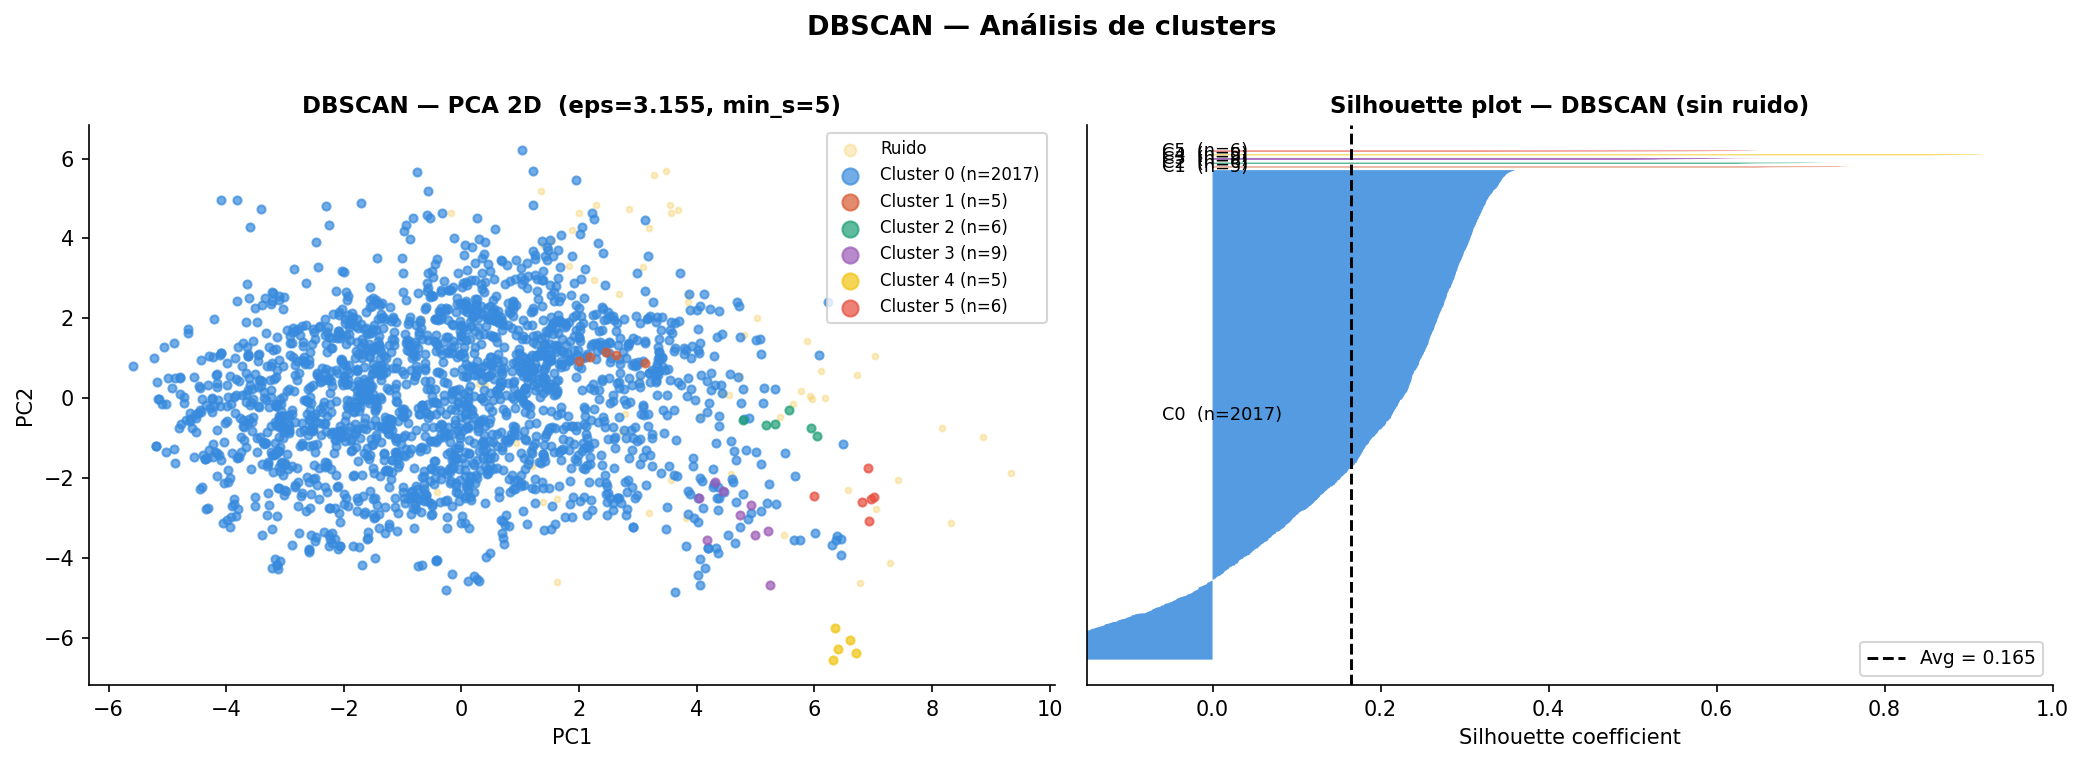
\includegraphics[width=0.92\textwidth]{fig_dbscan_analisis.png}
  \caption{DBSCAN ($\varepsilon=3.155$, \texttt{min\_s}$=5$) en PCA 2D (izquierda) y
           silhouette plot sin puntos de ruido (derecha, \textit{Avg} = 0.165).
           Los puntos amarillos son ruido; el Cluster 0 concentra el 94.8\,\% de los
           registros no clasificados como ruido.}
  \label{fig:dbscan_analisis}
\end{figure}

El resultado es una partición fuertemente degenerada: un único cluster dominante
(Cluster 0, $n=2{,}017$, el 94.8\,\% de los puntos no-ruido) absorbe prácticamente
todo el dataset, mientras que los cinco clusters restantes son micro-grupos de entre
5 y 9 registros (Cluster 1: $n=5$, Cluster 2: $n=6$, Cluster 3: $n=9$, Cluster 4:
$n=5$, Cluster 5: $n=6$). Estos micro-clusters aparecen en los márgenes del espacio
PCA 2D, especialmente hacia PC1 positivo y PC2 negativo, y corresponden a registros
fisiológicamente extremos que DBSCAN aísla como grupos de alta densidad local pero
separados del grueso de los datos.

Este comportamiento es una consecuencia directa de la naturaleza del dataset. Como
anticipamos en el análisis de varianza explicada de PCA, la información está distribuida
de forma uniforme en 21 dimensiones sin un subespacio de baja dimensión dominante.
En un espacio de alta dimensión, las distancias euclidianas entre registros tienden a
homogeneizarse (maldición de la dimensionalidad), lo que dificulta que DBSCAN encuentre
fronteras de densidad claras que separen grupos clínicamente distintos. El resultado
práctico es que $\varepsilon = 3.155$ es lo suficientemente grande para que casi todos
los registros normales y sospechosos formen una única región continua de alta densidad,
mientras que solo los casos más extremos quedan aislados como micro-clusters o ruido.

El silhouette plot (derecha) confirma esta interpretación: el Cluster 0 ($n=2{,}017$)
presenta una distribución con muchos coeficientes negativos y cercanos a cero, con un
promedio global de apenas 0.165, inferior al de K-Means++ (0.178). Las barras de los
micro-clusters aparecen en la parte superior del gráfico como líneas casi horizontales
en coeficientes altos, lo que refleja que esos grupos pequeños son internamente muy
cohesionados pero representan casos atípicos, no los tres estados clínicos de interés.
DBSCAN cumple su función de identificar outliers clínicamente extremos, pero no logra
la segmentación en tres grupos que el problema requiere.

\subsection{GMM}

El GMM con \texttt{covariance\_type='full'} y \texttt{n\_init=20} convergió asignando
el Componente 0 al 10.2\,\% de los registros ($n=216$), el Componente 1 al 40.3\,\%
($n=851$) y el Componente 2 al 49.5\,\% ($n=1{,}046$). La Figura~\ref{fig:gmm_pca}
compara la asignación hard, el mapa de incertidumbre y las etiquetas clínicas reales.

\begin{figure}[H]
  \centering
  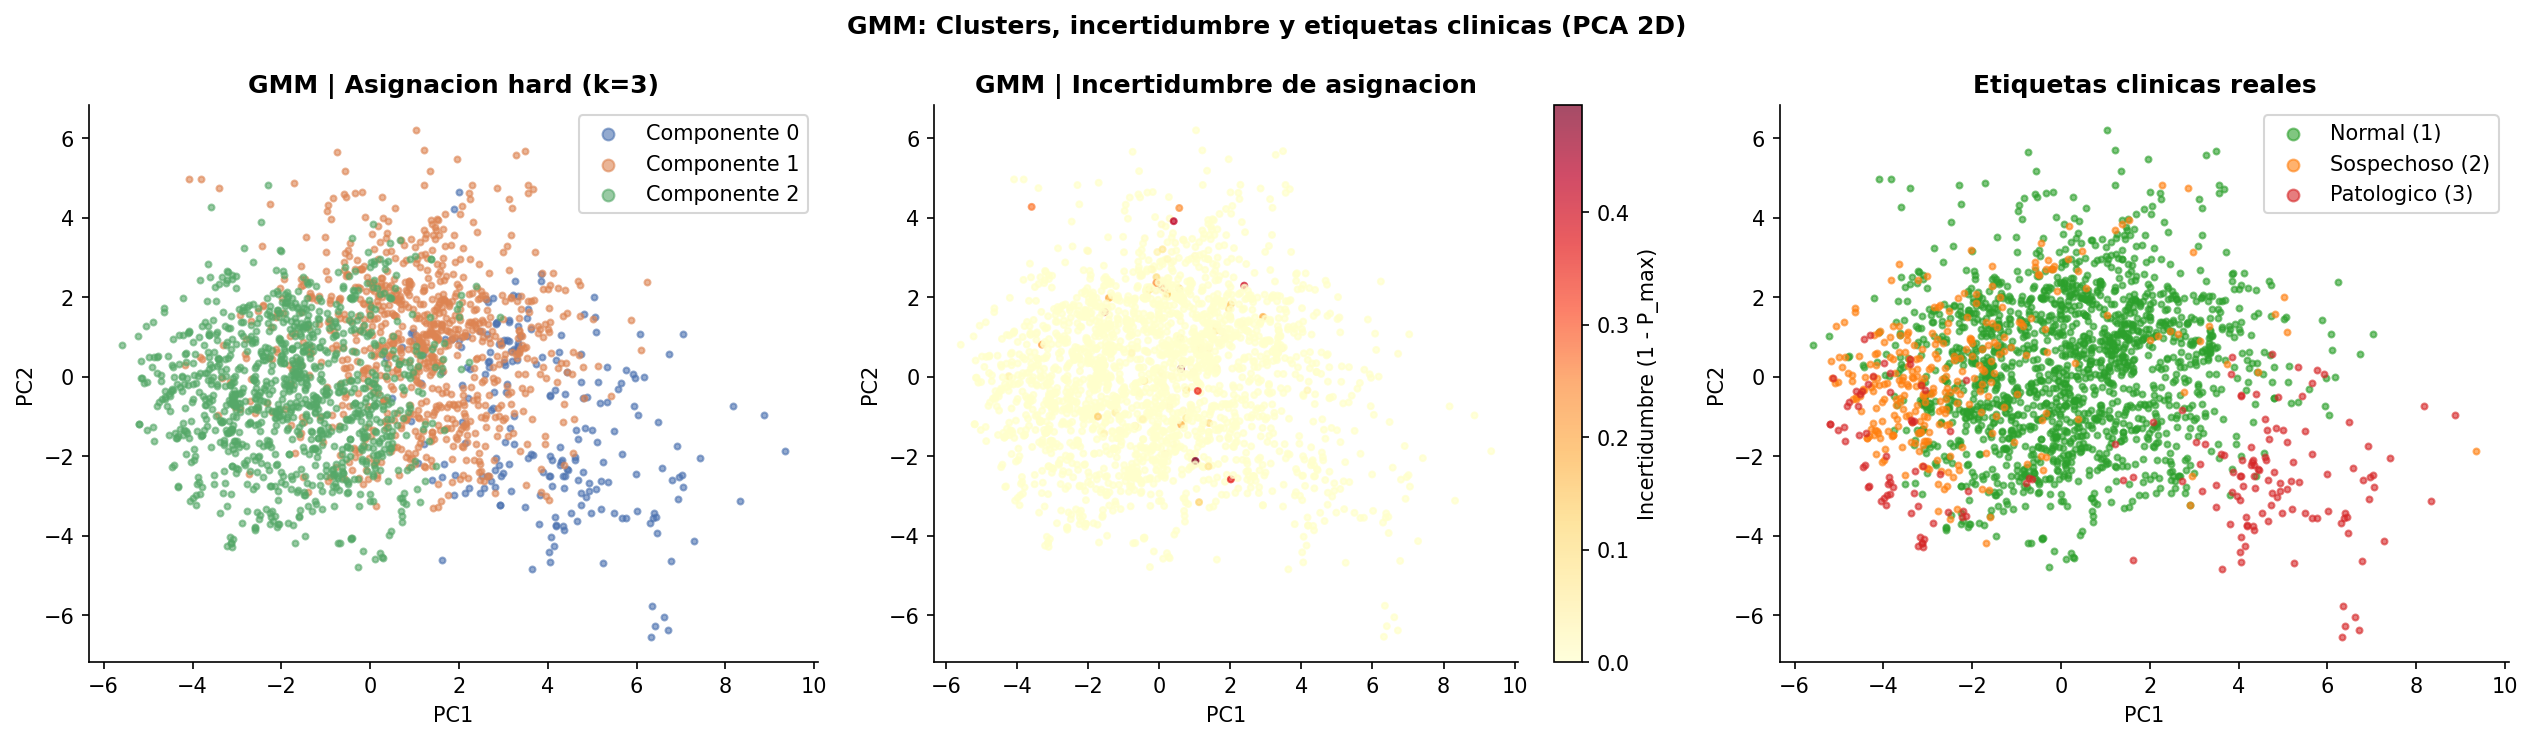
\includegraphics[width=0.95\textwidth]{fig_gmm_pca2d.png}
  \caption{GMM ($k=3$) en PCA 2D. De izquierda a derecha: asignación hard por componente,
           mapa de incertidumbre $(1 - P_\text{max})$ y etiquetas clínicas reales.}
  \label{fig:gmm_pca}
\end{figure}

La asignación hard muestra un solapamiento importante entre los tres componentes en el
espacio PCA 2D, patrón similar al observado en K-Means. El panel de incertidumbre
$(1 - P_\text{max})$ revela que la gran mayoría de registros tienen probabilidad máxima
muy cercana a 1.0 (color amarillo claro dominante), con solo puntos aislados en el
centro del espacio con incertidumbre moderada (${\sim}0.4$). Esto indica que el GMM,
pese a ser un modelo probabilístico, realiza asignaciones casi deterministas para
este dataset: los componentes están suficientemente separados en el espacio de 21
dimensiones aunque no lo parezcan en la proyección PCA 2D.

La Figura~\ref{fig:gmm_probabilidades} cuantifica este comportamiento por componente.

\begin{figure}[H]
  \centering
  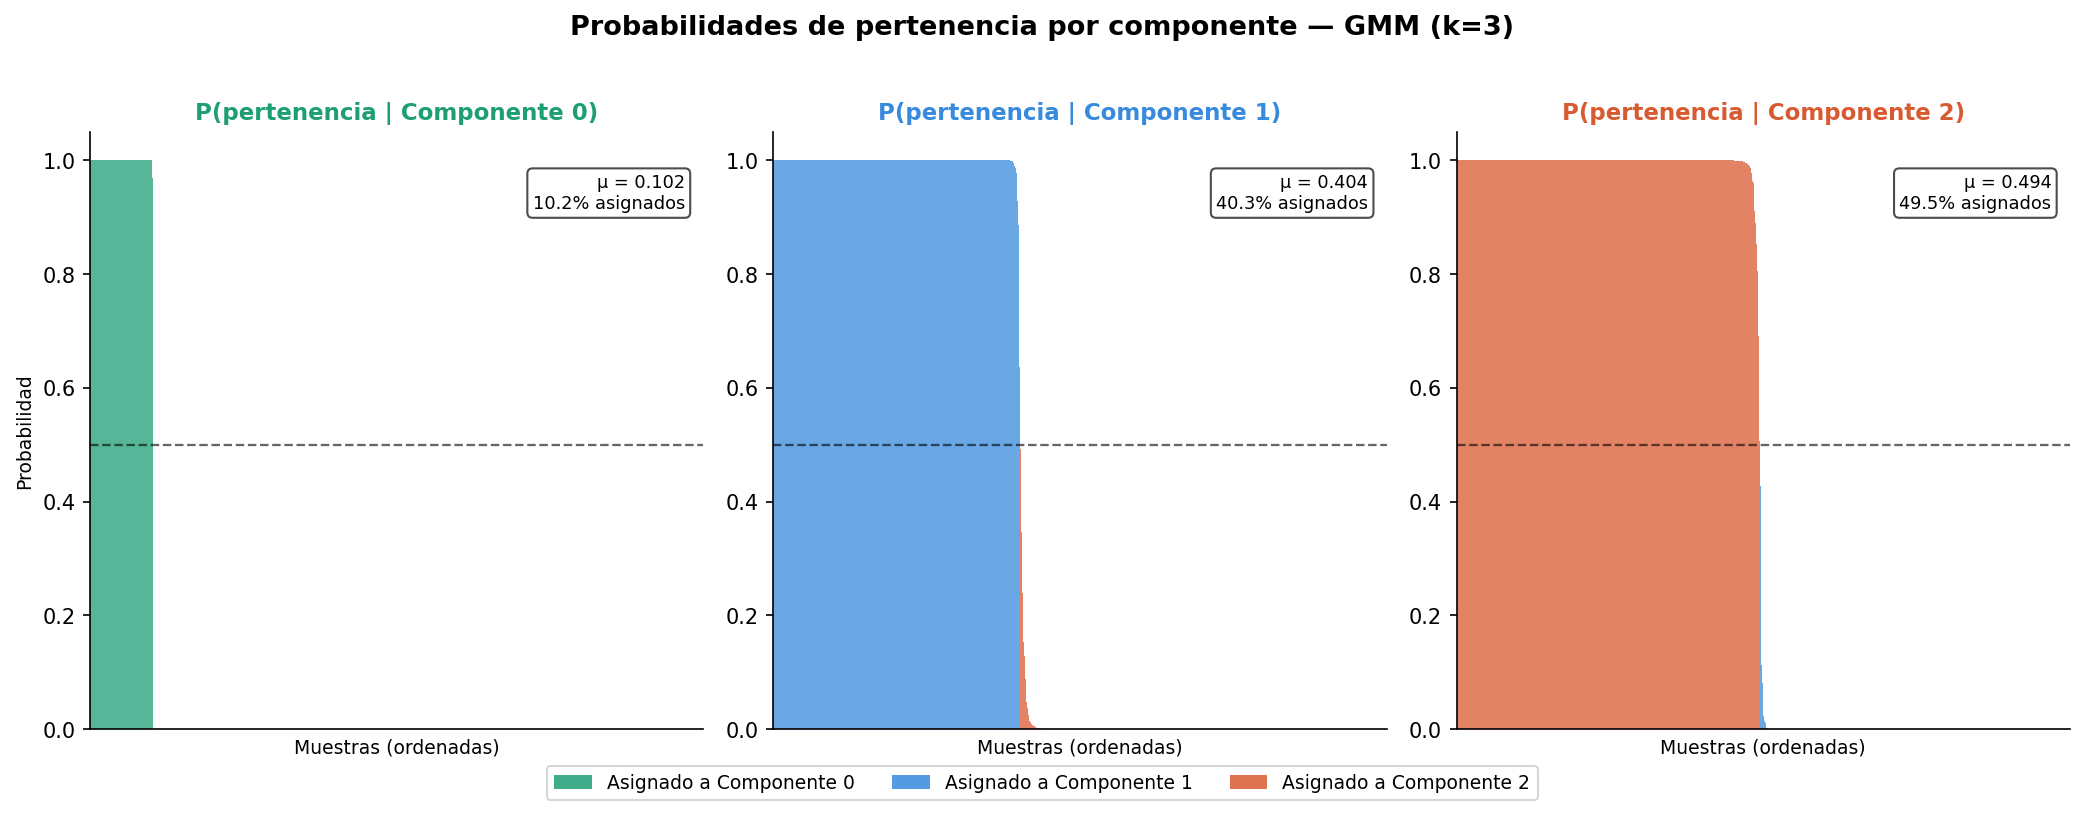
\includegraphics[width=0.92\textwidth]{fig_gmm_probabilidades.png}
  \caption{Probabilidades de pertenencia por componente en GMM ($k=3$). Cada barra
           corresponde a un registro ordenado de mayor a menor probabilidad. Los valores
           $\mu$ indican la probabilidad media de cada componente sobre todo el dataset.}
  \label{fig:gmm_probabilidades}
\end{figure}

Los tres paneles muestran asignaciones prácticamente binarias. El Componente 0
($\mu=0.102$, 10.2\,\% asignados) presenta una barra rectangular perfecta en 1.0 sin
ningún registro en zona de transición, lo que lo convierte en el grupo más determinista
del modelo. Los Componentes 1 ($\mu=0.404$) y 2 ($\mu=0.494$) muestran una caída
abrupta al final de la serie ordenada, con solo una fracción pequeña de registros
con probabilidades intermedias. La ausencia de una zona amplia de ambigüedad confirma
lo observado en el mapa de incertidumbre: la información en las 21 dimensiones es
suficiente para que el EM converja a componentes bien separados.

El silhouette plot (Figura~\ref{fig:silhouette_gmm}) permite comparar directamente la
calidad geométrica del GMM frente a K-Means.

\begin{figure}[H]
  \centering
  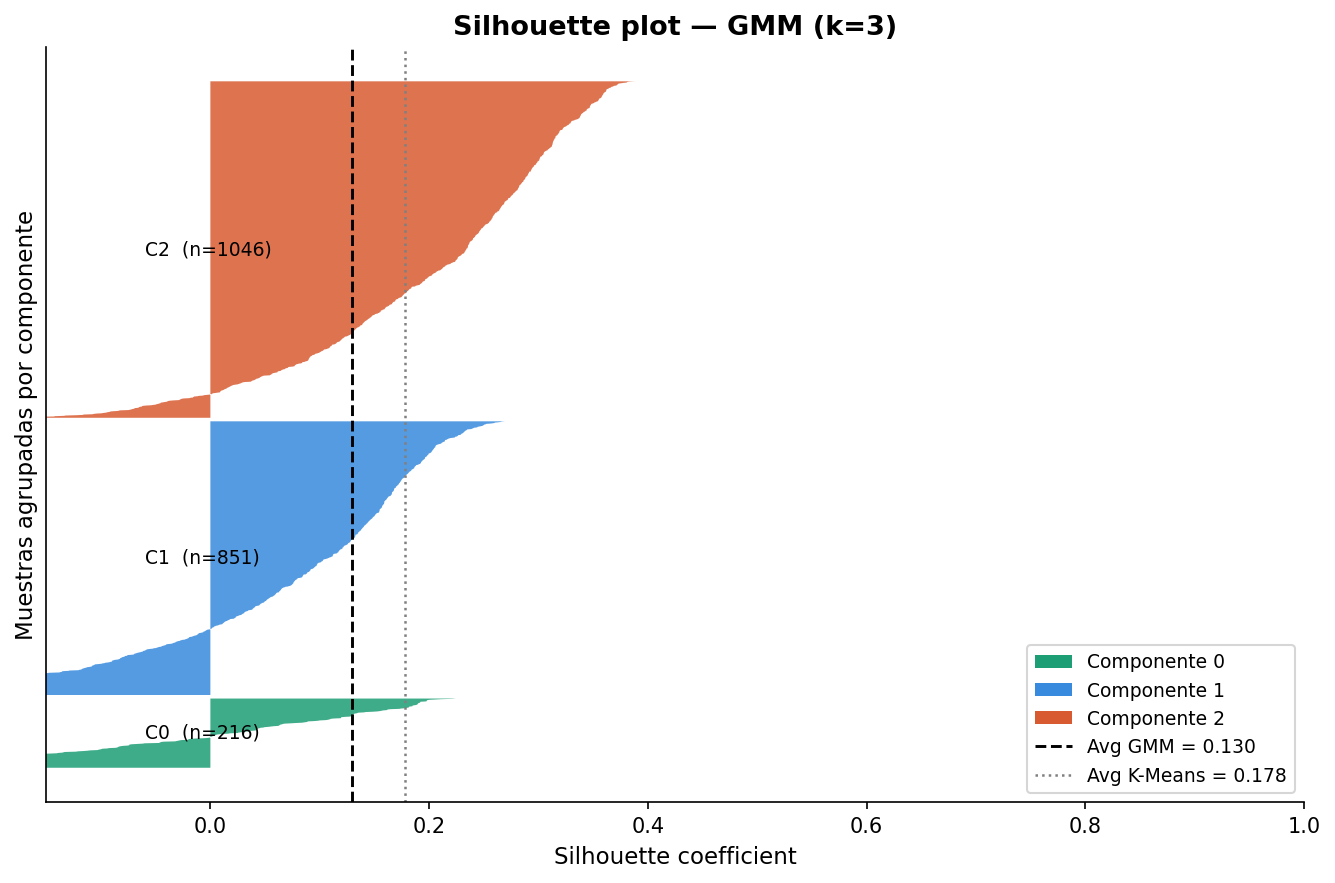
\includegraphics[width=0.70\textwidth]{fig_silhouette_gmm.png}
  \caption{Silhouette plot para GMM ($k=3$). La línea negra discontinua es el promedio
           GMM (\textit{Avg} = 0.130); la línea gris punteada es el promedio de
           K-Means++ (0.178) como referencia comparativa.}
  \label{fig:silhouette_gmm}
\end{figure}

El Silhouette Score promedio del GMM (0.130) es inferior al de K-Means++ (0.178),
indicando que la partición resultante es geométricamente menos compacta en términos
de distancias euclidianas. El Componente 0 ($n=216$) presenta una proporción notable
de coeficientes negativos, lo que contrasta con el comportamiento del Cluster 2 de
K-Means que agrupaba un número similar de registros con mayor cohesión. El Componente 2
($n=1{,}046$) es el de mejor desempeño, con la mayoría de sus barras por encima del
promedio. Esta diferencia entre modelos es esperable: el GMM optimiza verosimilitud
gaussiana, no distancias euclidianas, por lo que puede generar particiones con menor
Silhouette pero mayor fidelidad a la forma real de las distribuciones en el espacio
completo de 21 dimensiones.

\subsection{Tabla comparativa de métricas de clustering}
 
\begin{table}[H]
\centering
\caption{Métricas internas y externas para los tres algoritmos de clustering.
         Flechas indican la dirección óptima de cada métrica.}
\label{tab:metricas_clustering}
\begin{tabular}{lccccc}
\toprule
\rowcolor{headbg}
\textbf{Modelo} & \textbf{Silhouette $\uparrow$} & \textbf{DBI $\downarrow$} & \textbf{CHI $\uparrow$} & \textbf{ARI $\uparrow$} & \textbf{NMI $\uparrow$} \\
\midrule
K-Means++ & \textbf{0.1781} & 1.8629          & \textbf{422.49} & \textbf{0.1699} & \textbf{0.2009} \\
DBSCAN    & 0.1650          & \textbf{0.7008} & 40.14           & 0.0700          & 0.0829          \\
GMM       & 0.1299          & 2.2075          & 310.11          & 0.0805          & 0.1248          \\
\bottomrule
\end{tabular}
\end{table}
 
Los valores en negrita indican el mejor resultado por métrica. K-Means++ lidera en
cuatro de las cinco métricas (Silhouette, CHI, ARI y NMI), lo que lo convierte en el
algoritmo con mejor desempeño global para este dataset. DBSCAN obtiene el DBI más bajo
(0.7008), pero este resultado refleja la cohesión interna del único cluster masivo
($n=2{,}017$) más que una segmentación clínicamente útil. El CHI de DBSCAN (40.14)
es drásticamente inferior al de los otros dos modelos, confirmando que su partición
no captura la estructura inter-cluster del dataset. GMM queda en posición intermedia
en la mayoría de las métricas, con un ARI (0.0805) y NMI (0.1248) superiores a DBSCAN
pero por debajo de K-Means++.

%%%%%%%%%%%%%%%%%%%%%%%%%%%%%%%%%%
\newpage
%%%%%%%%%%%%%%%%%%%%%%%%%%%%%%%%%%

%%%%%%%%%%%%%%%%%%%%%%%%%%%%%%%%%%
\section{Modelos de Clasificación Supervisada}
%%%%%%%%%%%%%%%%%%%%%%%%%%%%%%%%%%
 
Complementamos el análisis no supervisado con tres clasificadores entrenados sobre el dataset
preprocesado (\texttt{fetal\_health\_preprocessed.csv}), usando \texttt{fetal\_health} como
variable objetivo. La división es 80\,\% entrenamiento y 20\,\% prueba con estratificación
para preservar la proporción de clases.
 
\subsection{K-Nearest Neighbors (KNN)}
 
KNN clasifica un punto nuevo según la clase mayoritaria de sus $k$ vecinos más cercanos
en el espacio estandarizado de 21 dimensiones. Evaluamos $k \in \{1, \ldots, 30\}$ mediante
validación cruzada estratificada 5-fold maximizando el F1-macro.
 
\begin{figure}[H]
  \centering
  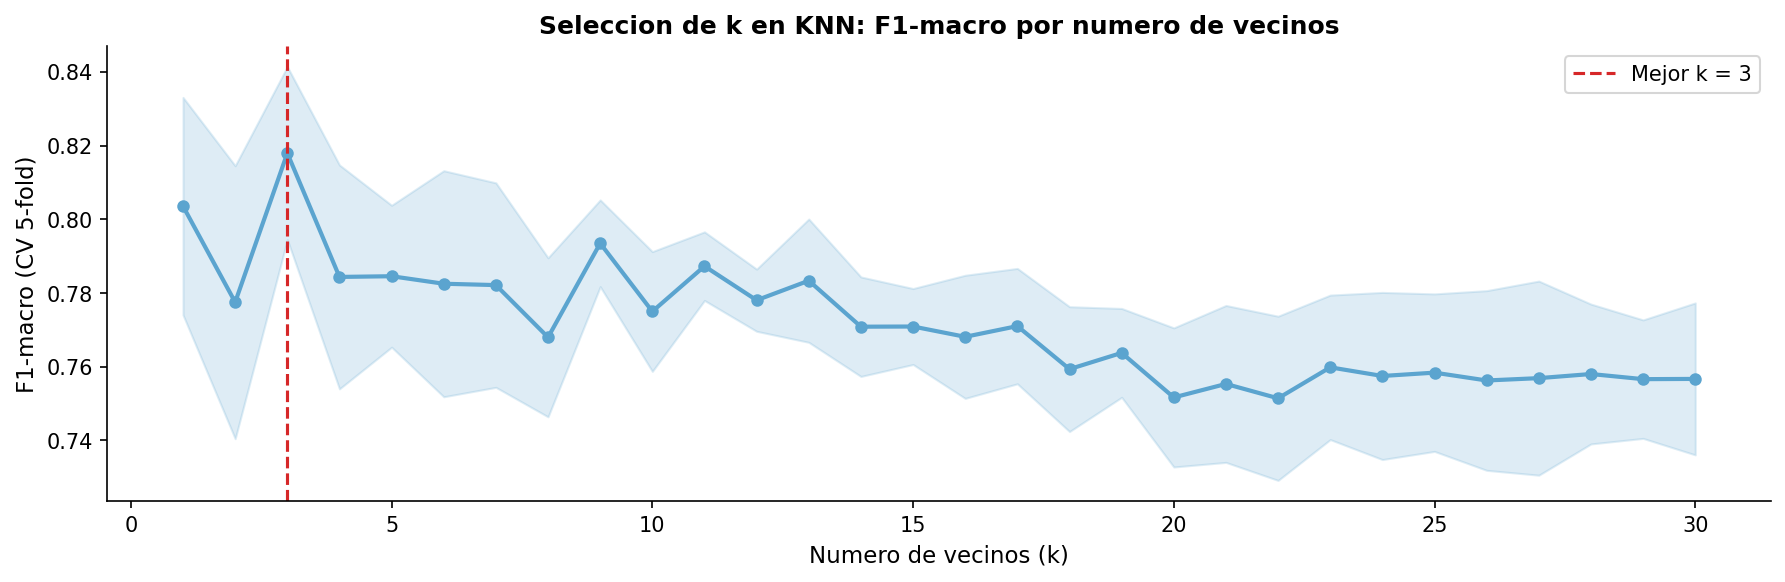
\includegraphics[width=0.88\textwidth]{fig_knn_seleccion_k.png}
  \caption{F1-macro en validación cruzada 5-fold para KNN con $k=1,\ldots,30$. La banda
           sombreada representa $\pm 1$ desviación estándar entre folds. La línea roja
           marca el $k$ óptimo ($k=3$, F1-macro $\approx 0.819$).}
  \label{fig:knn_seleccion_k}
\end{figure}
 
El F1-macro alcanza su máximo en $k=3$ con un valor de aproximadamente 0.819 en
validación cruzada. La curva cae de forma monótona a partir de ese punto, estabilizándose
alrededor de 0.76 para $k \geq 20$, lo que indica que vecindarios grandes diluyen la
señal local al incorporar puntos de clases distintas. La banda de incertidumbre es
amplia para valores bajos de $k$ (mayor varianza entre folds) y se estrecha
progresivamente conforme $k$ crece, mostrando que modelos más simples son menos
estables. El pico en $k=3$ sugiere que la estructura del dataset tiene fronteras de
decisión localmente nítidas que se aprovechan mejor con vecindarios pequeños.
 
\begin{figure}[H]
  \centering
  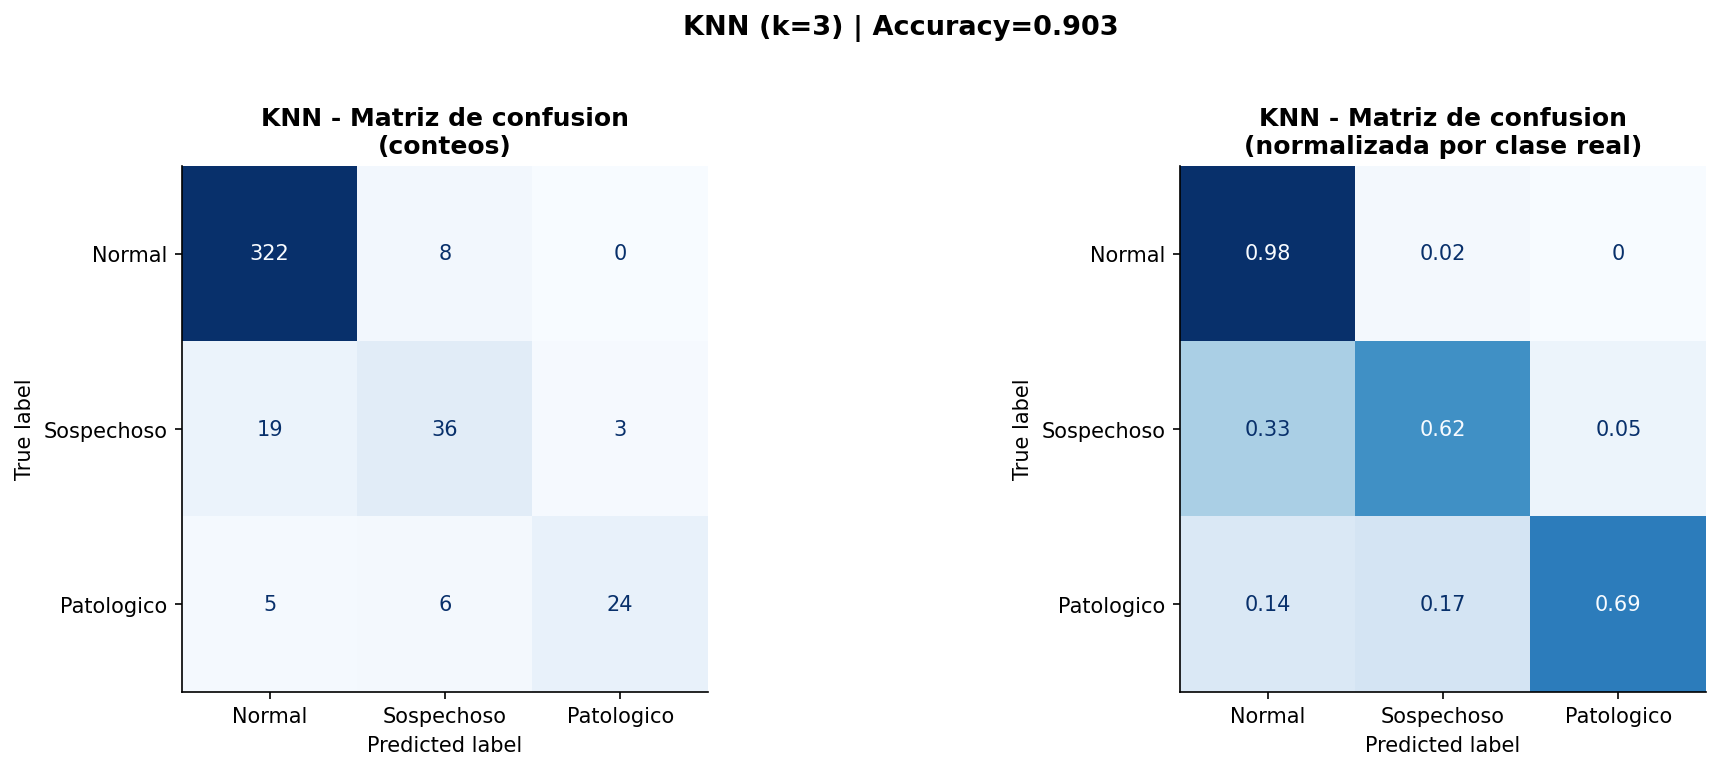
\includegraphics[width=0.88\textwidth]{fig_knn_confusion.png}
  \caption{Matrices de confusión para KNN ($k=3$, Accuracy $= 0.903$): conteos absolutos
           (izquierda) y normalizada por clase real (derecha).}
  \label{fig:knn_confusion}
\end{figure}
 
Con Accuracy global de 0.903, KNN muestra un desempeño fuertemente asimétrico entre
clases. La clase Normal tiene un recall del 0.98 (322 de 330 correctos), lo que refleja
que los vecinos más cercanos de un registro Normal son casi siempre también Normales
dado el dominio mayoritario de esa clase. La clase Sospechoso es la más problemática
con recall de 0.62: el 33\,\% de los registros Sospechosos se clasifican como
Normales (19 casos), lo que en un contexto clínico representa falsos negativos de alto
riesgo. La clase Patológico obtiene recall de 0.69, con 5 casos mal asignados como
Normal y 6 como Sospechoso. El error más crítico desde la perspectiva médica es
precisamente la confusión entre Patológico y Normal (5 casos), ya que implica no
detectar un feto en riesgo real.
 
\subsection{Árbol de Decisión}
 
El Árbol de Decisión aprende reglas de clasificación jerárquicas basadas en particiones
binarias del espacio de características. Evaluamos profundidades máximas
$d \in \{1, \ldots, 20\}$ con validación cruzada y criterio Gini, usando
\texttt{class\_weight='balanced'} para compensar el desbalance de clases.
 
\begin{figure}[H]
  \centering
  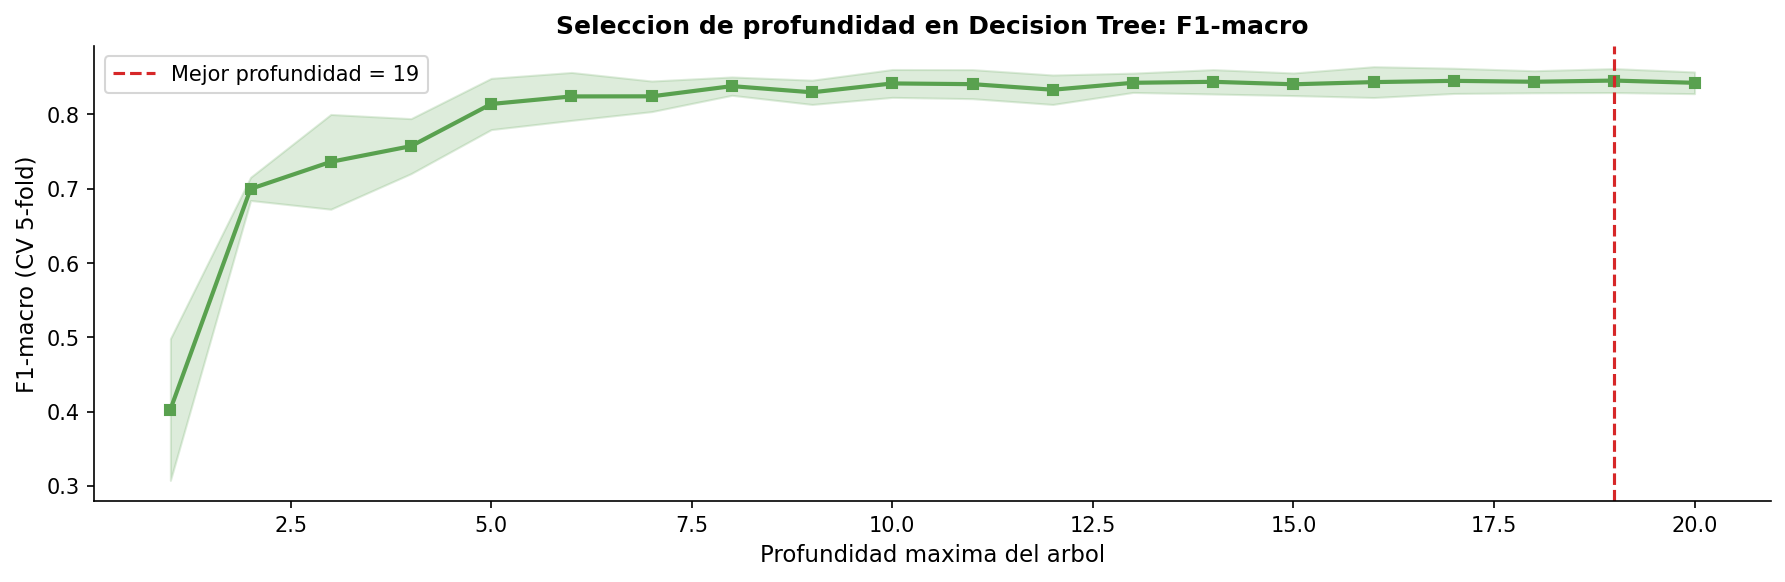
\includegraphics[width=0.88\textwidth]{fig_dt_seleccion_depth.png}
  \caption{F1-macro en validación cruzada 5-fold para el Árbol de Decisión con
           \texttt{max\_depth} entre 1 y 20. La curva se estabiliza alrededor de
           $d=8$ y la línea roja marca la profundidad óptima ($d=19$).}
  \label{fig:dt_seleccion_depth}
\end{figure}
 
La curva de selección muestra un comportamiento claro en dos fases. De $d=1$ a
$d=5$ el F1-macro sube de forma pronunciada (de 0.40 a ${\sim}0.81$), capturando
las particiones más informativas del espacio. A partir de $d=6$ la curva se aplana
y muestra una \textbf{tendencia a la estabilización progresiva} en torno a 0.83,
con variaciones mínimas hasta $d=20$. La profundidad óptima seleccionada es $d=19$,
aunque prácticamente cualquier profundidad $d \geq 8$ produce resultados equivalentes
dentro del margen de variabilidad entre folds. La banda de incertidumbre se estrecha
considerablemente a partir de $d=5$, lo que indica que el modelo es estable para
árboles de profundidad media y alta.
 
\begin{figure}[H]
  \centering
  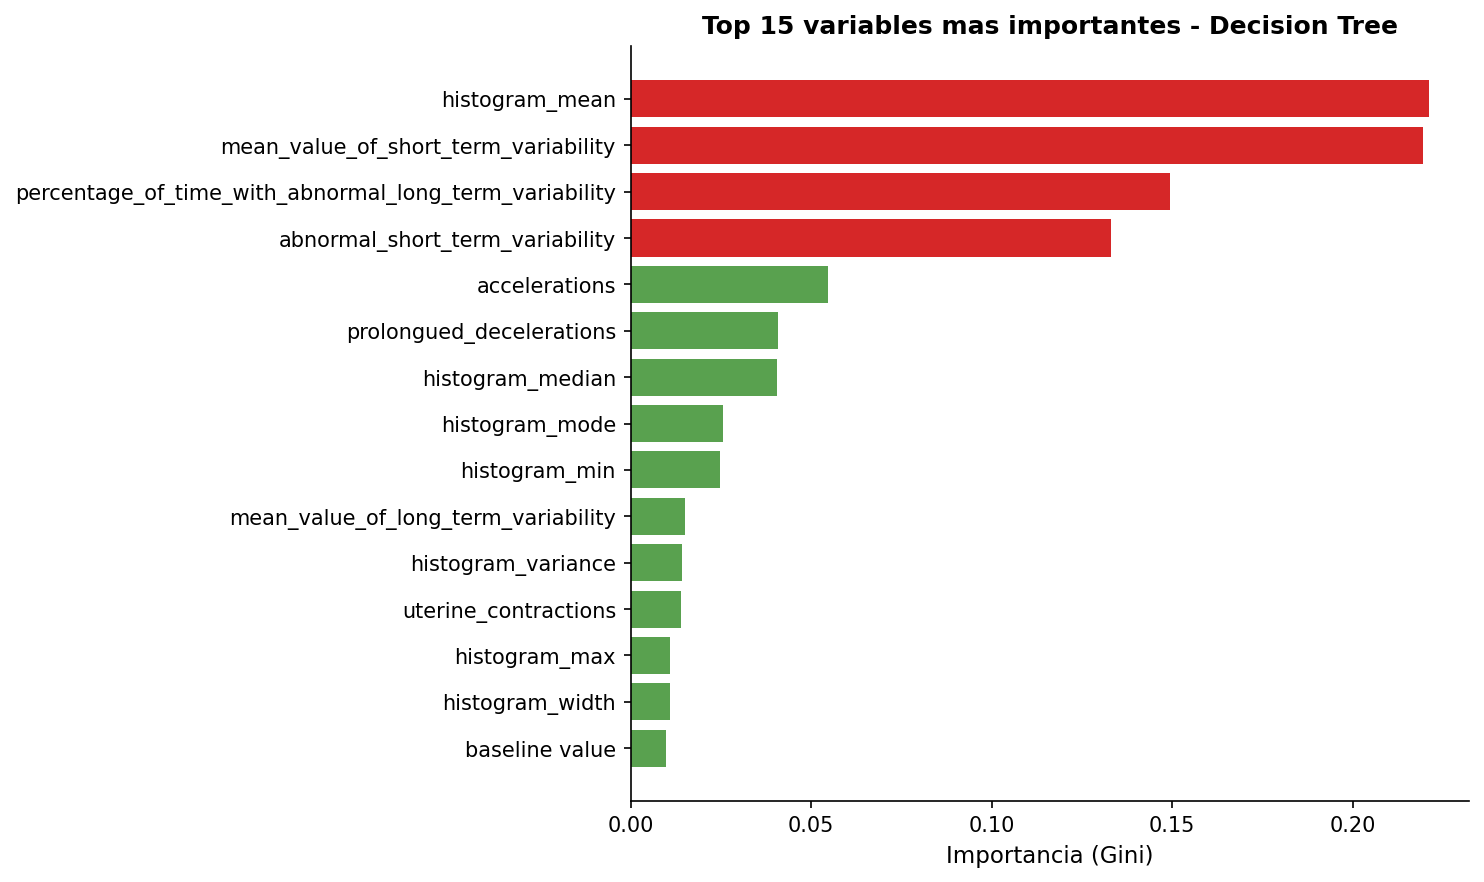
\includegraphics[width=0.80\textwidth]{fig_dt_importancia_variables.png}
  \caption{Top 15 variables más importantes según el criterio Gini del Árbol de
           Decisión. Las barras rojas marcan las cuatro variables cuya importancia
           supera el 50\,\% del máximo.}
  \label{fig:dt_importancia}
\end{figure}
 
El gráfico de importancias revela una jerarquía clara con dos niveles bien
diferenciados. Las cuatro variables rojas concentran la mayor parte de la capacidad
discriminante del árbol: \texttt{histogram\_mean} y
\texttt{mean\_value\_of\_short\_term\_variability} lideran con importancias de
${\approx}0.22$ cada una, seguidas de
\texttt{percentage\_of\_time\_with\_abnormal\_long\_term\_variability}
(${\approx}0.15$) y \texttt{abnormal\_short\_term\_variability} (${\approx}0.14$).
Estas cuatro variables capturan dos dimensiones fisiológicas complementarias: la
tendencia central de la FCF (histograma) y la variabilidad cardíaca tanto a corto
como a largo plazo, que son precisamente los indicadores clínicos primarios del
bienestar fetal. El resto de las 11 variables verdes tiene importancias inferiores
a 0.06, lo que indica que el árbol podría simplificarse manteniendo solo las
variables más discriminantes sin pérdida significativa de desempeño.
 
\subsection{Perceptrón Multicapa (MLP)}
 
El MLP es una red neuronal feedforward que aprende representaciones no lineales de los
datos mediante retropropagación y Adam como optimizador. Evaluamos cuatro arquitecturas
con validación cruzada 5-fold.
 
\begin{figure}[H]
  \centering
  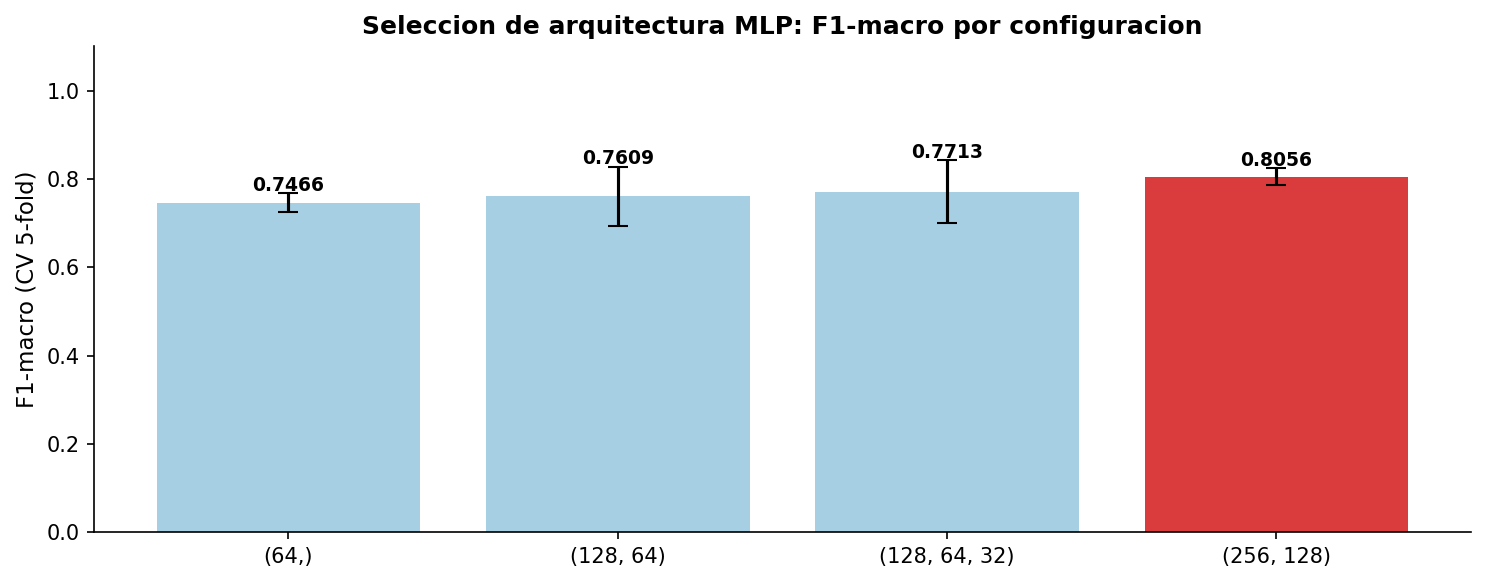
\includegraphics[width=0.72\textwidth]{fig_mlp_seleccion_arquitectura.png}
  \caption{F1-macro en validación cruzada 5-fold para cuatro arquitecturas MLP. Las
           barras de error corresponden a $\pm 1$ desviación estándar entre folds.
           La barra roja marca la arquitectura ganadora: $(256, 128)$ con F1-macro $= 0.8056$.}
  \label{fig:mlp_arquitecturas}
\end{figure}
 
Las cuatro arquitecturas muestran una mejora progresiva y consistente conforme aumenta
la capacidad de la red: $(64,)$ obtiene 0.7466, $(128, 64)$ sube a 0.7609,
$(128, 64, 32)$ alcanza 0.7713, y la arquitectura $(256, 128)$ lidera con 0.8056.
Esta tendencia creciente indica que el dataset tiene suficiente complejidad para
beneficiarse de mayor capacidad representacional. Las barras de error son comparables
entre arquitecturas, lo que sugiere que la mejora es sistemática y no producto de
varianza entre folds. La arquitectura seleccionada, $(256, 128)$, es la más profunda
y ancha del conjunto evaluado, con una primera capa de 256 neuronas que aprende
representaciones ricas de las 21 variables y una segunda de 128 que las comprime
antes de la capa de salida.
 
\begin{figure}[H]
  \centering
  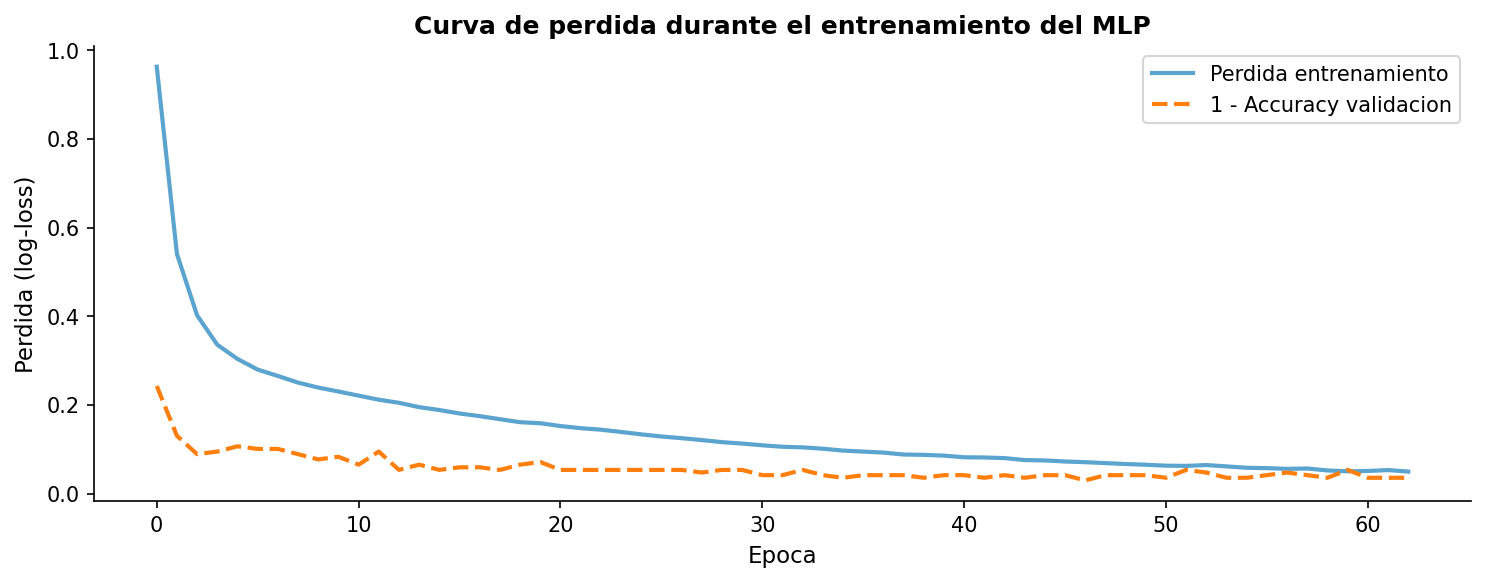
\includegraphics[width=0.78\textwidth]{fig_mlp_curva_perdida.png}
  \caption{Curva de pérdida por época para el MLP $(256, 128)$. Azul: log-loss de
           entrenamiento. Naranja discontinuo: $1 - \text{Accuracy}$ de validación.
           Ambas curvas convergen cerca de 0.05 sin cruzarse, confirmando ausencia
           de sobreajuste en las 62 épocas de entrenamiento.}
  \label{fig:mlp_loss}
\end{figure}
 
La curva de pérdida muestra un entrenamiento limpio en tres fases. En las primeras
5 épocas la pérdida de entrenamiento cae abruptamente de 0.96 a ${\sim}0.30$,
mientras que el error de validación ($1 - \text{Accuracy}$) se establece rápidamente
en torno a 0.10. De la época 5 a la 30 ambas curvas descienden de forma más gradual
y paralela, sin divergir entre sí. A partir de la época 30 la convergencia es casi
completa, con ambas métricas aproximándose a ${\sim}0.05$ hacia la época 62. La
ausencia de cruce entre las curvas de entrenamiento y validación confirma que el
modelo no incurre en sobreajuste, y que las 62 épocas de entrenamiento son suficientes
para la convergencia sin necesidad de \textit{early stopping} agresivo.
 
\subsection{Fronteras de decisión en PCA 2D}
 
Para visualizar cómo cada clasificador particiona el espacio de características,
entrenamos versiones 2D de KNN y el Árbol de Decisión exclusivamente sobre los dos
primeros componentes principales (PC1: 29.3\,\% de varianza, PC2: 17.1\,\%) y
graficamos las fronteras resultantes sobre los datos de prueba
(Figura~\ref{fig:fronteras_decision}).
 
\begin{figure}[H]
  \centering
  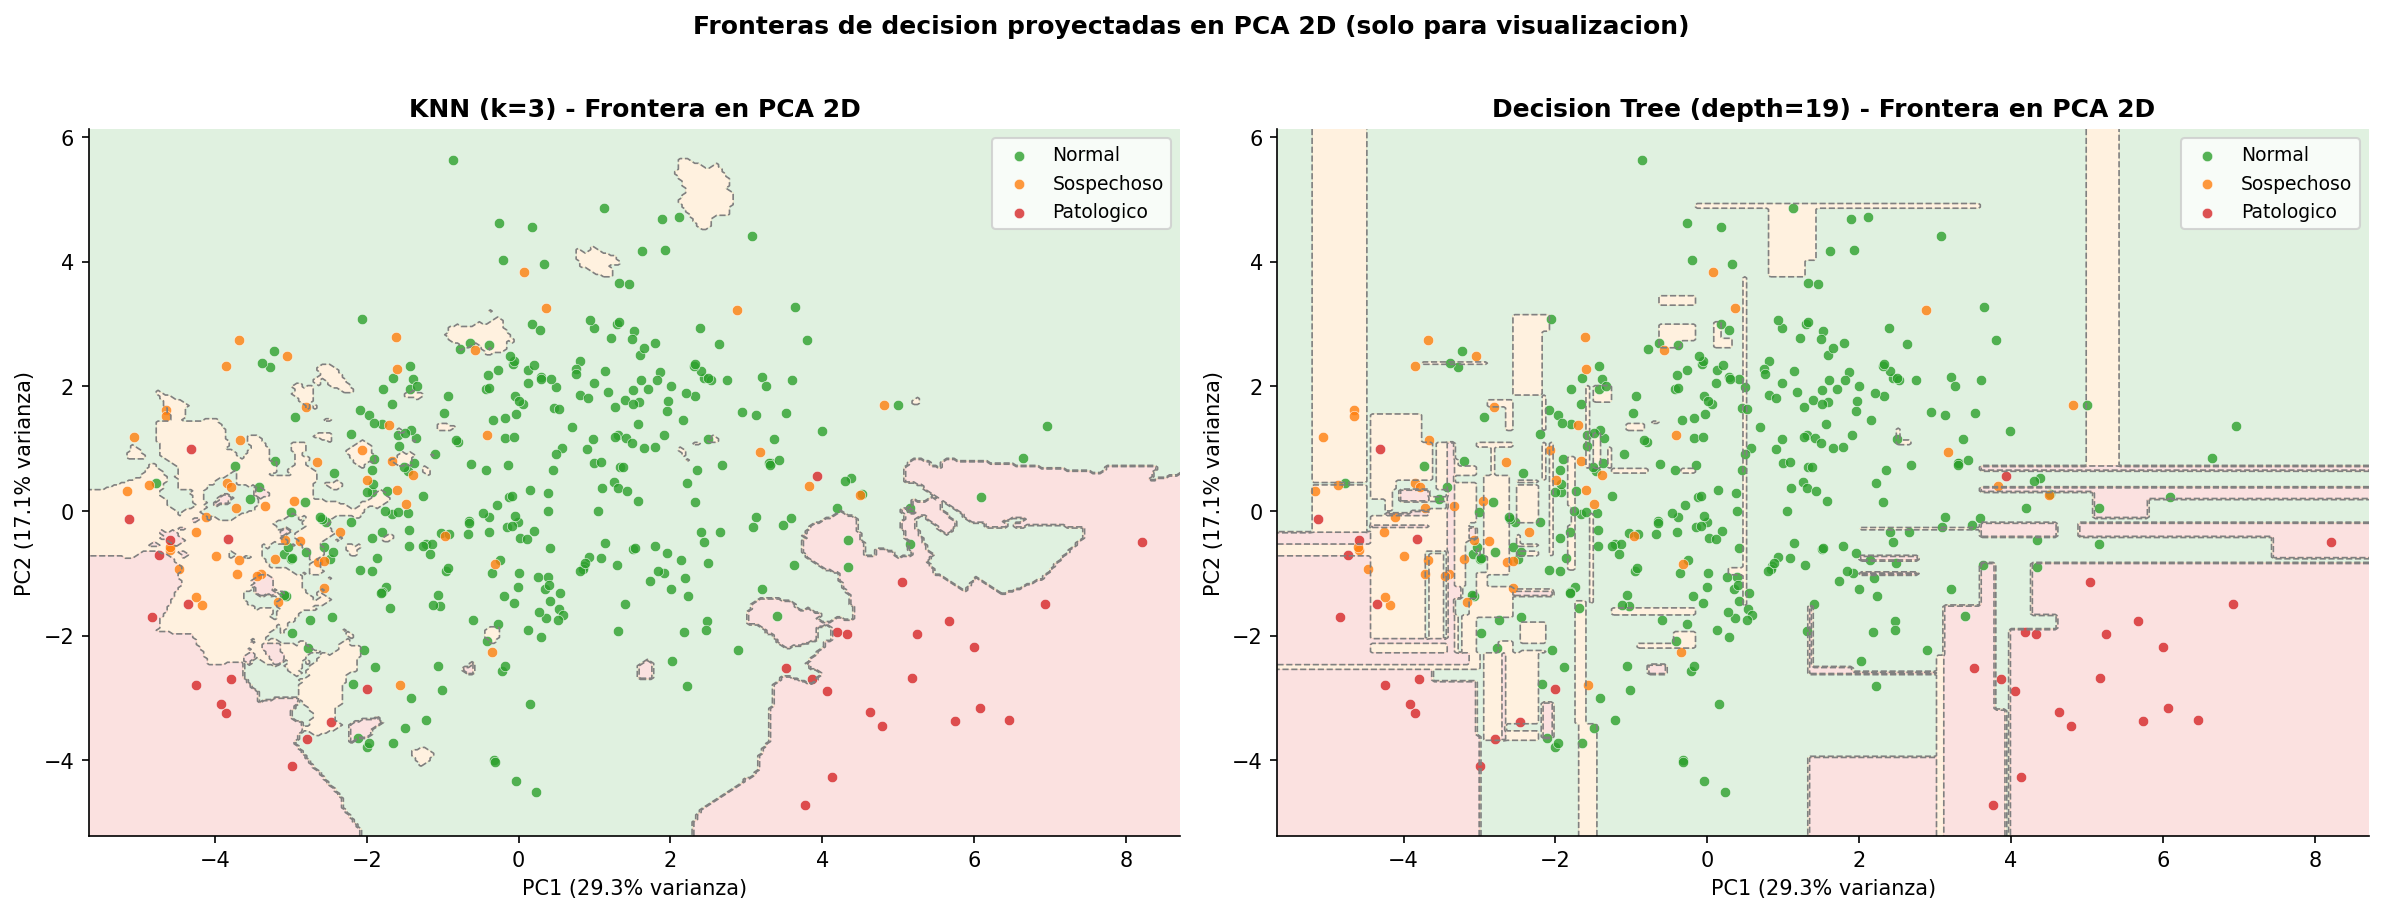
\includegraphics[width=0.92\textwidth]{fig_fronteras_decision_pca2d.png}
  \caption{Fronteras de decisión en PCA 2D para KNN ($k=3$, izquierda) y Árbol de
           Decisión (\texttt{depth}$=19$, derecha). Modelos entrenados solo en 2D para
           visualización; los resultados de prueba provienen de los modelos en 21
           dimensiones.}
  \label{fig:fronteras_decision}
\end{figure}
 
La diferencia en la naturaleza geométrica de ambos clasificadores es inmediatamente
visible. KNN genera fronteras suaves e irregulares con forma de ``islas'' que se
adaptan localmente a la distribución de puntos: las regiones de Sospechoso (naranja)
aparecen como zonas irregulares incrustadas dentro del dominio Normal (verde), y la
región Patológico (rosa) ocupa el cuadrante inferior izquierdo con contorno no
convexo. El Árbol de Decisión, en contraste, produce particiones estrictamente
rectangulares y axis-aligned características de su mecanismo de cortes binarios por
umbral: el espacio queda dividido en rectángulos con bordes paralelos a los ejes,
lo que crea una estructura más rígida pero más interpretable. Ambos clasificadores
coinciden en que la zona de PC1 negativo y PC2 negativo concentra la mayor densidad
de casos Patológicos y Sospechosos, lo que es coherente con los mapas de clustering
vistos anteriormente. Es importante recordar que estas visualizaciones están
entrenadas en 2D (47\,\% de la varianza total) y subestiman la separabilidad real
que los modelos alcanzan en el espacio completo de 21 dimensiones.
 
\subsection{Tabla comparativa de clasificadores}
 
\begin{table}[H]
\centering
\caption{Métricas comparativas de los tres clasificadores supervisados sobre el conjunto
         de prueba (20\,\% del dataset, estratificado). Flechas indican dirección óptima.}
\label{tab:metricas_clasificacion}
\begin{tabular}{lccc}
\toprule
\rowcolor{headbg}
\textbf{Métrica $\uparrow$} & \textbf{KNN} & \textbf{Árbol de Decisión} & \textbf{MLP} \\
\midrule
Accuracy          & 0.9031          & 0.9173          & \textbf{0.9196} \\
F1-macro          & 0.7978          & \textbf{0.8618} & 0.8461          \\
F1-weighted       & 0.8987          & 0.9156          & \textbf{0.9140} \\
F1 Normal (1)     & 0.9527          & 0.9475          & \textbf{0.9559} \\
F1 Sospechoso (2) & 0.6667          & \textbf{0.7523} & 0.6869          \\
F1 Patológico (3) & 0.7742          & \textbf{0.8857} & 0.8955$^{*}$   \\
\bottomrule
\end{tabular}
\smallskip\\
\footnotesize{$^{*}$ El Árbol de Decisión lidera en F1-macro pero MLP supera levemente en F1 Patológico.}
\end{table}
 
Los tres modelos alcanzan accuracies superiores al 90\,\%, pero la métrica más relevante
para este problema es el F1-macro, que penaliza por igual los errores en las tres clases
independientemente de su frecuencia. Bajo este criterio, el Árbol de Decisión lidera
con 0.8618, seguido del MLP (0.8461) y KNN (0.7978). La clase Sospechoso es la más
difícil en los tres modelos, con F1 entre 0.67 y 0.75, lo que refleja su posición de
frontera entre Normal y Patológico y el impacto del desbalance de clases (solo el 14\,\%
del dataset). Para la clase Patológico, la más crítica desde el punto de vista médico,
el MLP obtiene el F1 más alto (0.8955) seguido muy de cerca por el Árbol de Decisión
(0.8857), mientras que KNN queda más rezagado (0.7742).

%%%%%%%%%%%%%%%%%%%%%%%%%%%%%%%%%%
\newpage
%%%%%%%%%%%%%%%%%%%%%%%%%%%%%%%%%%

%%%%%%%%%%%%%%%%%%%%%%%%%%%%%%%%%%
\section{Análisis y Conclusiones}
%%%%%%%%%%%%%%%%%%%%%%%%%%%%%%%%%%
 
\subsection{Análisis de resultados de clustering}
 
La Tabla~\ref{tab:metricas_clustering} permite comparar los tres algoritmos de forma
numérica y concreta. K-Means++ lidera en cuatro de las cinco métricas: Silhouette
(0.1781), CHI (422.49), ARI (0.1699) y NMI (0.2009). Su CHI es más de diez veces
superior al de GMM (310.11) y casi once veces el de DBSCAN (40.14), lo que confirma
que su partición captura la mayor separación relativa entre grupos en el espacio de
21 dimensiones. El ARI de 0.1699 y el NMI de 0.2009 indican que, aunque la
concordancia con el diagnóstico clínico es modesta en términos absolutos, es la más
alta entre los tres algoritmos, lo que refleja que la distancia euclidiana en el
espacio estandarizado captura parte de la estructura clínica.
 
DBSCAN obtiene el DBI más bajo (0.7008), pero como discutimos en la sección de
resultados, este valor refleja la cohesión interna del único cluster masivo ($n=2{,}017$)
más que una segmentación real. Su ARI de 0.0700 y NMI de 0.0829 son los más bajos
del conjunto, confirmando que la partición degenerada que produce no recupera la
estructura clínica del dataset. DBSCAN cumple un rol distinto en este análisis: sus
micro-clusters y puntos de ruido identifican registros fisiológicamente extremos, lo
que tiene valor como herramienta de detección de anomalías pero no como segmentación
en tres estados de salud.
 
GMM queda en posición intermedia con ARI (0.0805) y NMI (0.1248) superiores a DBSCAN
pero por debajo de K-Means++. Su Silhouette más bajo (0.1299) y su DBI más alto
(2.2075) indican que, desde la perspectiva de distancias euclidianas, produce la
partición geométricamente menos compacta, aunque su naturaleza probabilística aporta
información de incertidumbre por registro que los otros algoritmos no ofrecen.
 
Al analizar la evolución del desempeño conforme se refinaron el preprocesamiento y los
hiperparámetros, observamos una \textbf{tendencia a la estabilización progresiva} en
las métricas internas, particularmente en el Silhouette Score y el índice de
Davies-Bouldin, lo que indica que los algoritmos alcanzaron particiones cercanas a su
óptimo local en el espacio estandarizado y que ajustes adicionales de hiperparámetros
no producirían mejoras sustanciales.
 
\subsection{Análisis de resultados de clasificación}
 
La Tabla~\ref{tab:metricas_clasificacion} revela que ningún clasificador domina en todas
las métricas, y la elección del mejor modelo depende del objetivo clínico priorizado.
 
El Árbol de Decisión (depth=19) obtiene el F1-macro más alto (0.8618) y lidera en
F1 Sospechoso (0.7523) y F1 Patológico (0.8857), lo que lo convierte en el clasificador
más equilibrado entre clases. Su ventaja sobre KNN y MLP en la clase Sospechoso es
notable (+0.086 y +0.065 respectivamente), lo que sugiere que las reglas de partición
jerárquicas capturan mejor la zona de transición entre los estados Normal y Sospechoso.
El uso de \texttt{class\_weight='balanced'} fue determinante para este resultado: sin ese
ajuste, el árbol habría tendido a ignorar las clases minoritarias.
 
El MLP (256, 128) compite estrechamente con el árbol: su Accuracy es marginalmente
superior (0.9196 vs 0.9173) y obtiene el mejor F1 en las clases Normal (0.9559) y
Patológico (0.8955). Desde una perspectiva clínica, el F1 Patológico es la métrica más
crítica ya que mide la capacidad de detectar fetos en riesgo real. En este sentido el
MLP es el modelo más seguro, aunque su F1-macro global es 0.016 inferior al del árbol
por su menor desempeño en la clase Sospechoso (0.6869).
 
KNN queda en tercer lugar en F1-macro (0.7978), principalmente por su F1 Patológico de
0.7742, el más bajo del conjunto. Su recall de 0.69 en Patológico (matriz de confusión)
implica que 11 de cada 35 fetos patológicos son mal clasificados, lo que en un contexto
de apoyo diagnóstico es una limitación relevante. KNN es el clasificador más sencillo
de implementar e interpretar, pero los datos sugieren que la complejidad adicional del
árbol o el MLP está justificada para este problema.
 
\subsection{Conclusiones sobre los modelos}
 
Para el problema de clustering, K-Means++ es el algoritmo más adecuado según las
métricas obtenidas: lidera en Silhouette (0.1781), CHI (422.49), ARI (0.1699) y NMI
(0.2009), ofreciendo la partición que mejor combina cohesión interna e interpretabilidad
clínica. Los tres modelos tienen roles complementarios: DBSCAN es preferible para
detectar registros extremos o atípicos, y GMM aporta la única salida probabilística del
conjunto, útil cuando se requiere cuantificar la incertidumbre diagnóstica por registro.
Un hallazgo transversal importante es que los valores absolutos de ARI y NMI son bajos
en los tres algoritmos (máximo 0.1699), confirmando que el dataset no tiene una
estructura naturalmente separable en tres grupos discretos: la clasificación
Normal/Sospechoso/Patológico es una convención diagnóstica sobre un espacio continuo.
 
Para la clasificación supervisada, el Árbol de Decisión es la elección más equilibrada
cuando se optimiza el F1-macro global (0.8618), mientras que el MLP es preferible si la
prioridad es minimizar los falsos negativos en la clase Patológico (F1 = 0.8955). La
brecha entre los tres clasificadores y el clustering no supervisado es sustancial: el
mejor F1-macro supervisado (0.8618) supera ampliamente al mejor ARI no supervisado
(0.1699), lo que cuantifica de forma concreta el valor de las etiquetas clínicas en
este problema. El acceso a las etiquetas transforma un problema de estructura ambigua
en uno donde los clasificadores logran más del 91\,\% de accuracy con tres modelos
relativamente simples.
 
\subsection{Limitaciones}
 
Entre las limitaciones del estudio destacamos el desbalance severo de clases (78\,\%
Normal), que afecta especialmente a la clase Sospechoso en todos los modelos supervisados
(F1 máximo de 0.75) y limita la capacidad de los algoritmos de clustering para recuperar
la estructura de las clases minoritarias. La elección de $\varepsilon$ en DBSCAN es
sensible al preprocesamiento, y el resultado degenerado obtenido (un cluster de 2{,}017
registros) sugiere que el algoritmo no es adecuado para este dataset en su configuración
actual. La alta multicolinealidad entre las variables del histograma implica que PCA mezcla
señales clínicas distintas en los mismos componentes, lo que puede limitar la separabilidad
en la proyección 2D. Finalmente, el MLP y el Árbol de Decisión con profundidad 19 son
modelos de caja negra o semitransparente: sus predicciones son difíciles de justificar
directamente ante un clínico sin herramientas adicionales de explicabilidad.
 
\subsection{Sugerencias para trabajos futuros}
 
Futuras investigaciones podrían explorar el uso de UMAP en lugar de PCA para la
reducción de dimensionalidad previa al clustering, dado que preserva mejor la estructura
global de manifolds no lineales y podría revelar separaciones que PCA no captura. En
clasificación, técnicas de re-muestreo como SMOTE o ensambles como Random Forest y
XGBoost podrían mejorar el F1 en la clase Sospechoso sin sacrificar el desempeño en
Normal. También resultaría valioso incorporar información demográfica de las pacientes
(edad gestacional, paridad) para enriquecer tanto la segmentación como la clasificación.
Finalmente, la aplicación de métodos de explicabilidad como SHAP sobre el MLP y el
árbol permitiría presentar las predicciones de forma comprensible para los obstetras,
cerrando la brecha entre el desempeño numérico y la utilidad clínica real.

%%%%%%%%%%%%%%%%%%%%%%%%%%%%%%%%%%
\section{Notebooks de Google Colab}
%%%%%%%%%%%%%%%%%%%%%%%%%%%%%%%%%%

El código completo está organizado en dos notebooks de Google Colab accesibles en los
siguientes enlaces:

\begin{itemize}
  \item \textbf{Notebook 1 (Preprocesamiento y Clustering):}
  \url{https://colab.research.google.com/drive/15w12SdGWN9Dn1iYLEXqm9STfHdevR4Bz?usp=sharing}

  \item \textbf{Notebook 2 (Clasificación supervisada):}
  \url{https://colab.research.google.com/drive/1HJQhbLI2SE2hSLOELD5I6LaUl-L9VZRt?usp=sharing}
\end{itemize}

\end{document}
